% Created 2019-10-08 Tue 22:15
% Intended LaTeX compiler: pdflatex
\documentclass[a4paper,11pt,openany]{book}
\usepackage[utf8]{inputenc}
\usepackage[T1]{fontenc}
\usepackage{graphicx}
\usepackage{grffile}
\usepackage{longtable}
\usepackage{wrapfig}
\usepackage{rotating}
\usepackage[normalem]{ulem}
\usepackage{amsmath}
\usepackage{textcomp}
\usepackage{amssymb}
\usepackage{capt-of}
\usepackage{hyperref}
\usepackage{helvet}
\usepackage{gensymb}
\usepackage{xcolor}
\usepackage{appendix}
\usepackage{tikz}
\usepackage{microtype}
\renewcommand{\familydefault}{\sfdefault}
\linespread{1.5}
\usepackage{tabularx}
\usepackage{tabu}
\usepackage[margin=1.4in]{geometry}
\usepackage[sort&compress,numbers]{natbib}
\usepackage[font=small,labelfont=bf]{caption}
\setcounter{secnumdepth}{2}
\author{\textbf{Student:} Jamin Wu \\ \textbf{Student ID:} 27025861 \\ \\ \textbf{Supervisor:} Dr Yan Tat Wong \\ \textbf{Co-Supervisor:} Dr Nicholas Price \\ \\ Department of Physiology \\ Department of Electrical \& Computer Systems Engineering \\ \textbf{School of Biomedical Sciences, Monash University} \\ \\ Minor thesis submitted in partial fulfillment of the requirements for the \\ degree Bachelor of Medical Science (Honours) at Monash University. \\ \\ Word Count: <> words}
\date{}
\title{\textbf{Using Generative Adversarial Networks to Derive Phosphene Patterns in Simulated Prosthetic Vision}}
\hypersetup{
 pdfauthor={\textbf{Student:} Jamin Wu \\ \textbf{Student ID:} 27025861 \\ \\ \textbf{Supervisor:} Dr Yan Tat Wong \\ \textbf{Co-Supervisor:} Dr Nicholas Price \\ \\ Department of Physiology \\ Department of Electrical \& Computer Systems Engineering \\ \textbf{School of Biomedical Sciences, Monash University} \\ \\ Minor thesis submitted in partial fulfillment of the requirements for the \\ degree Bachelor of Medical Science (Honours) at Monash University. \\ \\ Word Count: <> words},
 pdftitle={\textbf{Using Generative Adversarial Networks to Derive Phosphene Patterns in Simulated Prosthetic Vision}},
 pdfkeywords={},
 pdfsubject={},
 pdfcreator={Emacs 26.1 (Org mode 9.2.4)}, 
 pdflang={English}}
\begin{document}

\maketitle
\clearpage

\section*{Abstract}

\clearpage

\section*{Acknowledgements}

\clearpage

\section*{Declaration}

\clearpage

\setcounter{tocdepth}{3}
\tableofcontents

\chapter*{List of Abbreviations}

\begin{description}
\item[{CGAN}] conditional generative adversarial network
\item[{CVP}] cortical visual prosthesis
\item[{HPC}] high performance computing
\item[{GAN}] generative adversarial network
\item[{ReLU}] rectified linear unit
\end{description}

\listoftables
\listoffigures

\part{Background}
\label{sec:org9e45602}
\chapter{Introduction}
\label{sec:orgefd6405}

Blindness is a significant disability and can be caused by damage at any point along the visual pathway from the eye to the brain.
A \textbf{cortical visual prosthesis} (CVP) is a vision-restoring device inserted directly into the brain, replacing all parts of the visual pathway except the brain itself.
Because a CVP only requires a functioning brain, CVPs are a flexible (and potentially the only) option for many causes of non-cortical blindness.

However, a significant detractor from CVPs is that they are currently only expected to provide very low-quality vision.
As CVPs are still in early development with clinical trials only beginning to emerge, we still do not know exactly what people will be able to see.
What \emph{is} known is that people tend to see small spots of light called \textbf{phosphenes} - like "stars in a night sky" - when small regions of the brain are stimulated.
Unfortunately, we cannot yet reliably control the locations of phosphenes, nor their qualities beyond simply being "on" or "off".

To address the perceptual limitations of CVPs, a large body of research has been devoted to investigating how image processing techniques can make phosphenes meaningful.
These include using phosphenes to selectively display salient objects, display only prominent edges, or even replacing faces with low-resolution icons.
However, most of these studies are premised on static, optimistic simulations of prosthetic vision.
Many do not address how to apply traditional image processing strategies when we cannot control how phosphenes are laid out or what qualities they possess.
As a result, it is not clear what methods can be used to generalise image processing strategies to different people, who experience phosphenes differently.

Outside of prosthetic vision, there have been advances in using computers to generate novel imagery under specified conditions.
\textbf{Generative adversarial networks} (GANs) are a machine learning technique to generate new data samples (most often, images) when given many examples of data known prior.
GANs are not an image processing algorithm \emph{per se}, but a method of training a neural network to take a seed input and return a generated data sample.
GANs work by optimising the features of generated data samples to be as indistinguishable from real data samples as possible.
They have been used with varying degrees of success in a number of scene generation, style transfer and image processing tasks.

Because GANs are used to make generated images look more realistic, it is possible they could be used in a prosthetic vision setting to make phosphene patterns look more like what they are supposed to represent.
Importantly, GANs are a \emph{training} technique which can be applied to different types of phosphene simulations to produce specifically-tailored results.
This means GANs may be able to address the difficulties in finding generalised image processing strategies suitable for different people's experiences of prosthetic vision.

To our knowledge, there are no prior studies which attempt to apply GANs to the problems faced by prosthetic vision.
The following chapters review the literature surrounding CVPs, the visual percepts they produce, and previous approaches to addressing these limitations.

\chapter{Introduction}
\label{sec:orge2aef8c}

Around 36 million people worldwide were blind in 2015. \cite{bourne_magnitude_2017,flaxman_global_2017}
Many patients are left permanently blind when there is irreversible damage to the visual system such as from glaucoma or trauma. \cite{lee_glaucoma_2005,zachariades_blindness_1996}
However these patients often still have portions of the visual system intact, which could be leveraged to restore vision artificially.
\textbf{Cortical visual prostheses} are devices which aim to achieve exactly that - devices implanted on the brain which stimulate neurons to directly inject visual sensations into awareness. \cite{normann_toward_2009,lewis_restoration_2015,foroushani_cortical_2018}

Studies in the late 20th century showed that electrically stimulating the brain could indeed produce spot-like sensations of light, known as \textbf{phosphenes}. \cite{brindley_sensations_1968,dobelle_phosphenes_1974,bak_visual_1990,bosking_electrical_2017}
But these studies also revealed that we can exert only very limited control over what phosphenes look like, where they are located, and how they interact. \cite{rushton_properties_1978,dobelle_phosphenes_1974,schmidt_feasibility_1996}
Of these studies, those conducted in small groups also demonstrated wide variation in the appearance of phosphenes between people. \cite{dobelle_phosphenes_1974,bak_visual_1990}
Therefore, whilst we now know we can produce these spots of light by stimulating the brain, it is not clear how to assemble these unyielding percepts into useful vision for all implantees. \cite{fernandez_development_2005,beyeler_learning_2017}

To address this, new proposals of cortical visual prostheses are exploring the use of sophisticated computer processing to assemble phosphenes \emph{strategically} so implantees can interpret them in useful ways. \cite{foroushani_cortical_2018,barnes_role_2012}
These methods generally focus on addressing two significant difficulties of prosthetic vision: its low resolution, and its lack of color and brightness levels, both of which are easy to simulate on graphical displays and test.  \cite{buffoni_image_2005,chang_facial_2012,sharmili_comparative_2017}
However it is unclear how well these image processing algorithms could cope with the much wider range of phosphene experiences reported by perceptual studies in humans.
Thus, the primary issue facing these algorithms is how they can be made flexible to accommodate the large, uncontrollable variation in what phosphenes look like.

Recently, there have been remarkable advances in the ability of computers to \emph{derive} image processing algorithms rather than having algorithms being programmed by hand.
In this paradigm, computers iteratively "learn" and integrate patterns between data inputs and outputs through a process known as \textbf{machine learning}.  \cite{guo_deep_2016}
By using machine learning methods on top of layered image processing architectures called \textbf{convolutional neural networks} (CNNs) , computers are able to achieve near-human performance in image processing feats such as handwritten digit recognition \cite{ciresan_multi-column_2012}, segmenting images \cite{ciresan_deep_2012}, and replicating image styles. \cite{gatys_image_2016}
Machine learning principles could be similarly applied to prosthetic vision, using inferred patterns to derive image processing algorithms from performance rather than building algorithms around conceptions of what phosphenes look like.
This could improve the flexibility of cortical implants for different perceptual experiences and improve the usefulness of cortical visual prostheses for future implantees.


\clearpage

\chapter{What is a cortical visual prosthesis?}
\label{sec:orgfc938dd}
\label{org312a1bd}

\section*{Overview of Cortical Visual Prostheses}
\label{sec:org0217c50}

A \textbf{prosthesis} is an artificial, implanted device which aims to restore a lost function to the human body. \cite{thurston_pare_2007}
A \textbf{visual prosthesis} is such a device which aims to restore vision to people with visual impairment. \cite{weiland_visual_2008,ong_bionic_2012}
A \textbf{cortical visual prosthesis} specifically refers to a vision restoration device implanted on the cortical surface of the brain, as opposed to other portions of the visual system such as the eye, optic nerve or thalamus. \cite{lewis_restoration_2015}
As a cortical prosthesis is implanted directly on the brain, implantees only require a functional cortical portion of the visual system; the device bypasses any damage to the eyes or nerves leading up to the brain.
While visual prostheses at other locations in the visual pathway are also capable of producing visual sensations \cite{humayun_visual_1996,stingl_interim_2017,veraart_visual_1998,panetsos_consistent_2011}, their use-case, implementation and evoked vision differ from those produced by cortical prostheses and are outside the scope of this review.

Research into stimulating the brain to produce vision was first pioneered by Brindley \& Lewin \cite{brindley_sensations_1968} and later Dobelle \& Mladejovsky \cite{dobelle_phosphenes_1974} in the late 20th century.
Using rudimentary hardware, these early experiments showed that a temporary implant composed of a array of electrodes could stimulate the brain in an awake patient and make them see artificial sensations of light. \cite{brindley_sensations_1968,dobelle_phosphenes_1974}
These artificial sensations of light are known as \textbf{phosphenes}.
Phosphenes are highly variable, but most often appear as dots of light likened to "a star in the sky". \cite{dobelle_phosphenes_1974}
These early successes in evoking phosphenes were instrumental in demonstrating the feasibility of cortical prostheses \cite{schmidt_feasibility_1996}, which have adopted phosphenes as the fundamental building blocks of prosthetic vision.

In the past 50 years since, a small number of research groups have proposed modern cortical prostheses based on the principles of these early results.
These include the Gennaris bionic vision system \cite{lowery_restoration_2015,lowery_monash_2017}, the Intracortical Visual Prosthesis (ICVP) Project \cite{troyk_intracortical_2017}, CORTIVIS \cite{fernandez_cortivis_2017} and the Orion Visual Cortical Prosthesis. \cite{secondsight_second_nodate}
To illustrate what modern conceptions of a visual cortical prosthesis may look like, Figure \ref{fig:org1ac6c80} shows a simulated render of the headgear for the Gennaris bionic vision system.

\begin{figure}[htbp]
\centering
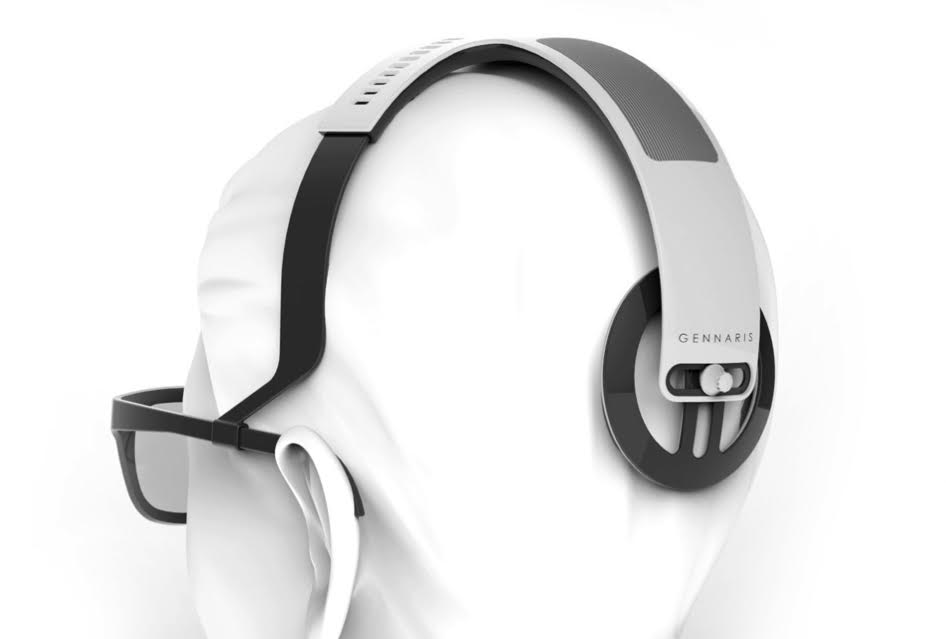
\includegraphics[width=.9\linewidth]{./graphics/litreview/headgear2.jpg}
\caption{\label{fig:org1ac6c80}
A modelled render of the Gennaris bionic vision headgear. Figure courtesy of Monash Vision Group.}
\end{figure}

These devices, while still early in development, may eventually be an option for restoring a crude form of vision to patients who would otherwise be left permanently blind.
The expectation is that these devices could provide gross light perception which might allow the recognition of basic forms and movement. \cite{lowery_monash_2017,lowery_restoration_2015}
Current technology cannot reproduce anything close to the trichromatic, approximately 15 million pixel resolution of the human eye \cite{deering_limits_1998}, and as such, these devices are not yet a full replacement for vision.
The development of specific cortical prostheses has been reviewed previously \cite{niketeghad_brain_2019}; we briefly summarise the current progress of these devices in Table \ref{tab:orgd498a04}.

\renewcommand{\arraystretch}{1.5}

\begin{table}[htbp]
\caption{\label{tab:orgd498a04}
Current progress of cortical visual prostheses. The number of electrodes places a hard upper bound on the resolution (and visual acuity) these devices can provide, so are noted here.}
\centering
\scriptsize
\begin{tabu} to \textwidth {XXXl}
Device & Electrodes & Progress & References\\
\hline
\textbf{Orion} \newline (Second Sight) & 60 subdural surface electrodes & FDA-approved clinical trial ongoing 2018-2023, six patients implanted (public scientific results yet to be released). & \cite{secondsight_early_nodate,secondsight_second_nodate,niketeghad_brain_2019}\\
\textbf{Gennaris} \newline (Monash Vision Group) & Up to 473 penetrating microelectrodes & Ethics approved to begin clinical trials, recruiting. & \cite{lowery_monash_2017,lowery_restoration_2015,anzctr_first_2018}\\
\textbf{ICVP Project} \newline (Illinois Institute of Technology) & 16 penetrating microelectrodes & Preclinical phase & \cite{troyk_intracortical_2017}\\
\textbf{CORTIVIS} \newline (Universidad Miguel Hernández) & 100 penetrating microelectrodes & Preclinical phase. & \cite{fernandez_cortivis_2017}\\
\end{tabu}
\end{table}

\section*{Mechanism of Cortical Visual Prostheses}
\label{sec:orgef7e32e}

While the specific hardware of each device differs, the fundamental mechanism of these devices is similar.
Patients must first undergo an operation to surgically implant an electrode array in the primary visual cortex at the back of the brain. \cite{lewis_restoration_2015}
Historically, these were subdural surface electrodes sitting atop (but not penetrating) the brain. \cite{brindley_sensations_1968,dobelle_phosphenes_1974}
However, modern prostheses tend to opt for penetrating microelectrodes \cite{lowery_monash_2017,troyk_intracortical_2017,fernandez_cortivis_2017} which are finer and can operate succesfully at lower electrical current. \cite{bak_visual_1990,schmidt_feasibility_1996}

After implantation, the physical components of the system are in place.
The system will need to be calibrated and tested before use to determine electrical stimulation thresholds and the spatial correpondence between electrodes and phosphenes in the visual fields. \cite{lowery_restoration_2015,fernandez_cortivis_2017}

When in use, an external camera (e.g. on glasses worn by the user) first captures an image. \cite{lowery_monash_2017,lewis_restoration_2015}
This image is transmitted to a portable processor, and is converted into electrical parameters for each electrode in the implanted array.
Each electrode in the implanted array then delivers pulses of electrical charge into the brain based on its parameters, which electrically stimulates nearby neurons in the cortical tissue.
Stimulating neurons in the visual cortex produces patterns of phosphenes which the patient can then perceive and interpret. \cite{brindley_sensations_1968,dobelle_phosphenes_1974,bak_visual_1990}
While these patterns may be difficult to decipher at first, it is expected that patients will eventually learn to match phosphene patterns to useful information such as letterforms. \cite{fernandez_cortivis_2017}

This process from camera image to neural stimulation loops continuously to produce a stream of images like frames of a video.
Essentially, this system provides an artificial real-time link between environmental light and visual information; a link ordinarily present in natural vision, but not present in blindness.
Figure \ref{fig:org99a3576} depicts the basic process of prosthetic vision in comparison to normal vision.

\begin{figure}[htbp]
\centering
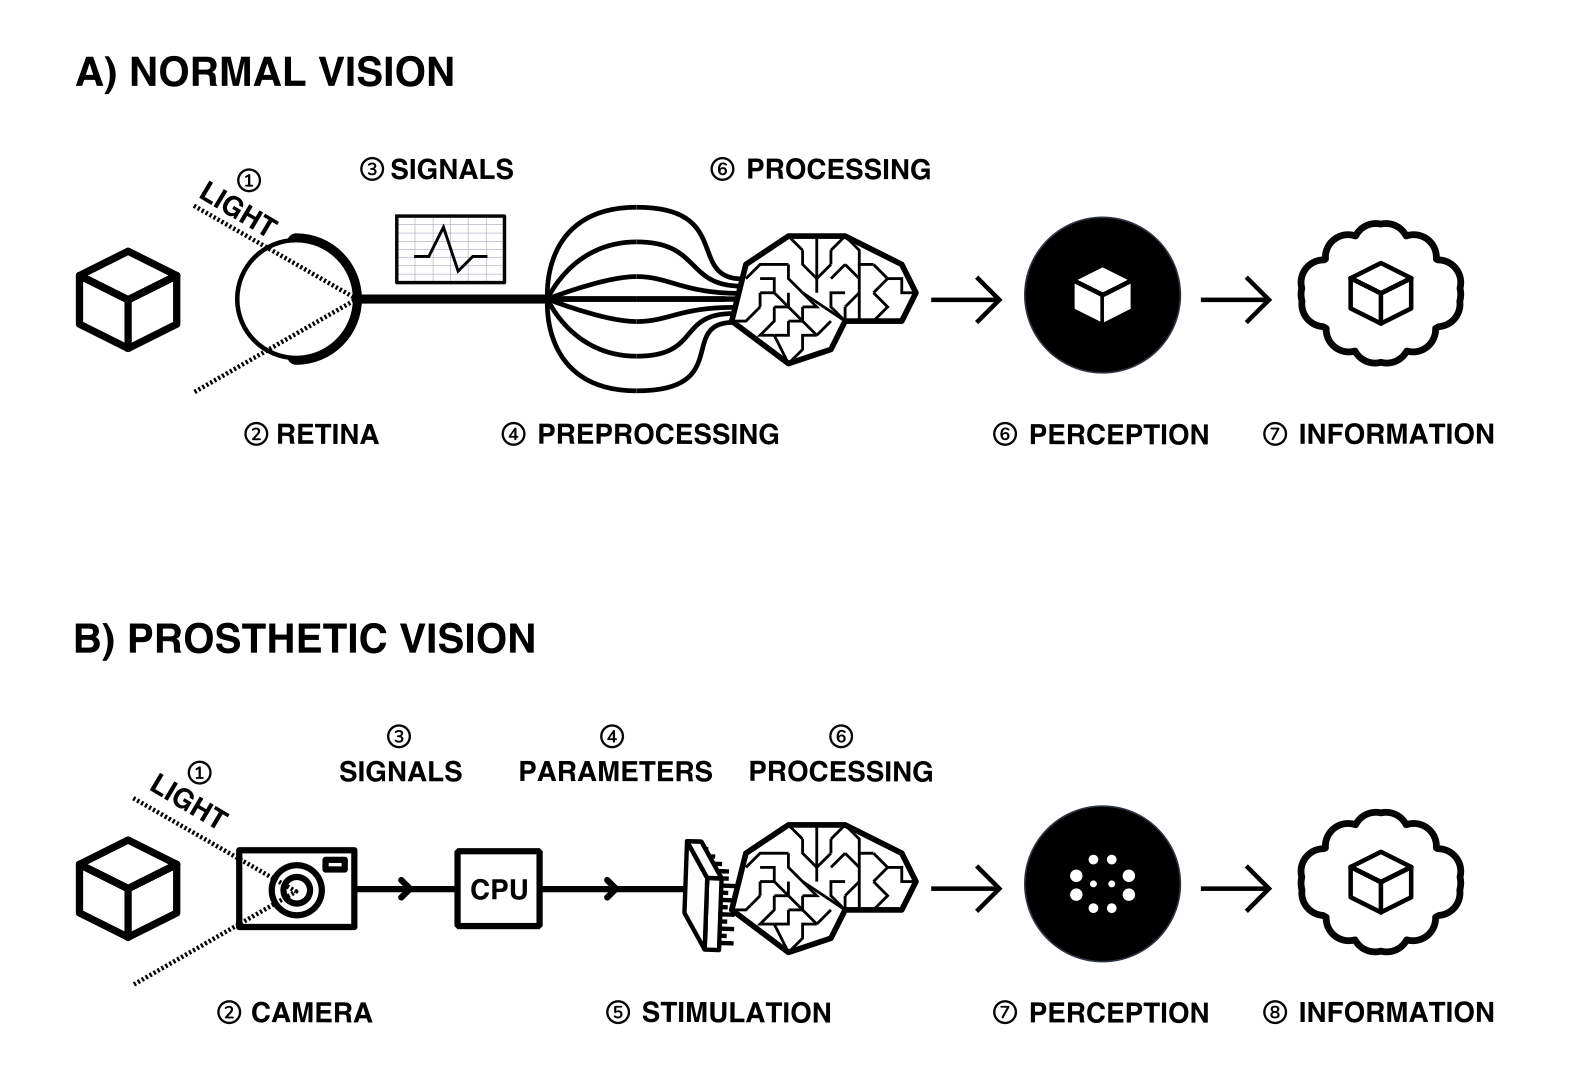
\includegraphics[width=.9\linewidth]{./graphics/litreview/flowchart.png}
\caption{\label{fig:org99a3576}
A basic flowchart of the process of prosthetic vision compared to normal vision. Figure made by the author.}
\end{figure}

\chapter{What do patients with cortical implants see?}
\label{sec:org6a0d704}
\label{org04debf3}

Because cortical visual prostheses use phosphenes as the fundamental building block of prosthetic vision, it is imperative that we be able to compose multiple phosphenes into meaningful imagery.
Whether phosphenes can be composed meaningfully depends on the visual and perceptual properties of phosphenes such as their size, color and interaction with other phosphenes.

Unfortunately, due to the technical and ethical issues surrounding stimulating peoples' brains, the number of studies characterising these properties of phosphenes in humans is understandably small.
Studies which characterise phosphenes evoked \emph{in vivo} typically fall into two distinct groups:

\begin{enumerate}
\item Historical experiments with rudimentary hardware on noble volunteers \cite{brindley_sensations_1968,dobelle_artificial_1974,bak_visual_1990}, or
\item Modern but conservative experiments in epilepsy patients who already have electrodes implanted for clinical monitoring. \cite{lee_mapping_2000,winawer_linking_2016,murphey_perceiving_2009,bosking_electrical_2017,collins_preserved_2019}
\end{enumerate}

As the pool of phosphene studies in humans is small and the demographics of these studies are skewed towards specific populations, we summarise the pertinent methodological features of each study in Table \ref{tab:orga4f277f}.
These studies constitute the major perceptual evidence that a cortical visual prosthesis can produce vision, and point towards what type of vision might be possible.

There are several studies which also attempt to characterise phosphenes in non-human primates from trained behavioural responses. \cite{tehovnik_phosphene_2005,tehovnik_phosphene_2007,tehovnik_microstimulation_2007,tehovnik_microstimulation_2009}
While the qualitative perceptual information offered by these studies is limited, they provide some additional information about the spatial properties of phosphenes inferred from sacaddes (rapid eye movements).

\linespread{1.1}
\newgeometry{margin=2cm}
\begin{sidewaystable}[htbp]
\caption{\label{tab:orga4f277f}
The participant demographics of studies which have looked at cortical phosphenes evoked \emph{in vivo} in humans.}
\centering
\scriptsize
\begin{tabu}{rlXX[2]X[2]X[2]}
Date & Reference & Setting & Electrodes & Parameters & Patient Demographic\\
\hline
1968 & \cite{brindley_sensations_1968} & Acute & 80 surface electrodes (array) on occipital cortex & Monophasic trains with 0.2ms pulses of unknown current (power 90mW) at 100Hz & 1 patient blind from  glaucoma and retinal detachment approx 1 year prior  (female, 52 years)\\
1974 & \cite{dobelle_phosphenes_1974} & Acute & Variable number of surface electrodes on occipial cortex & Monophasic or biphasic trains with 0.25-2ms/phase pulses of up to 1-5mA at 30-200Hz for 1000ms & 15 patients with cerebral tumours and partial visual field defects or normal sight (11 male, 4 female, 20-71 years)\\
1974 & \cite{dobelle_artificial_1974} & Acute & 64 subdural surface electrodes (array) on occipital cortex & Biphasic trains with 0.5ms/phase pulses of up to 8mA at 50Hz for unknown duration & 1 patient blind from congenital cataract in one eye and glaucoma and retinal detachment in the other for 28 years (male, 45 years); and 1 patient blind from trauma for 7 years (male, 28 years)\\
1978 & \cite{rushton_properties_1978} & Chronic \newline \{\tiny 5\textonehalf  years post implant\} & Unknown & Unknown-phase trains with with up to 2ms pulses of ?mA at 2-1000Hz for 1-8 pulses & Unknown\\
1976, 1979 & \cite{dobelle_braille_1976,dobelle_mapping_1979} & Chronic \newline \{\tiny unknown years post implant\} & 64 subdural surface electrodes (array) on occipital cortex & Biphasic trains with 0.25ms/phase pulses of 0.5-4.0mA at 50Hz for 500-1000ms & 1 patient blind from trauma 10 years prior to implantation (male, 33 and 35 years)\\
1990 & \cite{bak_visual_1990} & Acute & 1-3 intracortical penetrating microelectrodes on occipital cortex & Biphasic trains with 0.2ms/phase pulses of up to 200\(\mu\) A at 100Hz for 100-1000ms & 3 sighted patients with epilepsy (unknown demographic?)\\
1996 & \cite{schmidt_feasibility_1996} & Acute & 38 intracortical penetrating microelectrodes on occipital cortex & Biphasic trains with 0.2-0.8ms pulses of up to 80\(\mu\) A at 75-200Hz for 125-250ms & 1 patient blind from glaucoma 22 years prior (female, 42 years)\\
1994, 1999 & \cite{allison_face_1994,puce_electrophysiological_1999} & Acute & Unknown number of surface electrodes on extrastriate visual cortex & Biphasic trains with 0.2ms pulses of 2-10mA at 50Hz for 5000ms & Unknown\\
2000 & \cite{dobelle_artificial_2000} & Chronic \newline \{\tiny 21 years post implant\} & 64 (subdural?) surface electrodes (array) on on occipital cortex & Biphasic trains with 0.5ms/phase of (10-20V) at 30Hz for 1-50 pulses & 1 patient blind from trauma 5 years prior to implantation (male, 62 years)\\
2000 & \cite{lee_mapping_2000} & Acute & Total 271 subdural surface electrodes on occipital cortex and adjacent areas across all subjects & Biphasic trains with 0.3ms pulses of 1-15mA at 50Hz for 5000ms & 23 sighted patients with epilepsy (12 male, 11 female, 16-41 years)\\
2009 & \cite{murphey_perceiving_2009} & Acute & Total 50 subdural surface electrodes on 11 different visual areas across all subjects & Biphasic trains with 0.2ms pulses of 0.49-7mA at 200Hz for 300ms & 10 sighted patients with epilepsy (6 male, 4 female, 19-67 years)\\
2016 & \cite{winawer_linking_2016} & Acute & 1 or 2 subdural surface electrodes on V1 studied per subject & Biphasic trains with 0.2-1ms pulses of 0.2-5mA at 5-100Hz for 200-1000ms & 4 sighted patients with epilepsy (3 male, 1 female, 24-40 years)\\
2017 & \cite{bosking_saturation_2017} & Acute & Up to 16 subdural surface electrodes (array) on early occipital cortex per subject & Biphasic trains with 0.1ms/phase pulses of 0.3-4.0mA at 200Hz for 200-300ms & 15 sighted patients with epilepsy (5 male, 10 female, 22-61 years)\\
2018 & \cite{bosking_rules_2018} & Acute & Up to 16 subdural surface electrodes (array) on early occipital cortex per subject & Biphasic trains with 0.1ms/phase pulses of 0.3-4.0mA at 200Hz for 200-300ms & 8 sighted patients with epilepsy\\
2018 & \cite{beauchamp_dynamic_2018} & Acute & 16 or 24 subdural surface electrodes (array) on early occipital cortex per subject & Biphasic trains with 0.1ms/phase pulses of 0.3-4.0mA at 200Hz for 50-300ms & 4 sighted patients with epilepsy (all male, 20-54 years) and 1 patient blind 8 years prior, unspecified reason (female, 35 years)\\
2019 & \cite{collins_preserved_2019} & Acute & 16 subdural surface electrodes (array) on occipital cortex & Biphasic trains with 1ms pulses of up to 11mA at 60Hz & 1 patient with epilepsy and a partial visual fied defect for 30 years from AVM haemorrhage (male, 45 years)\\
\end{tabu}
\end{sidewaystable}
\restoregeometry
\linespread{1.5}

\section*{Phosphenes Produced by Stimulating a Single Electrode}
\label{sec:orga8dbe45}

The most common result of stimulating a single electrode is a single phosphene characterised as a small, localisable dot of light likened to a star. \cite{brindley_sensations_1968,dobelle_phosphenes_1974,schmidt_feasibility_1996,lee_mapping_2000}
Every study has, however, demonstrated large variation on this basic percept.

\subsection*{The Quality of a Phosphene}
\label{sec:org4471228}

Being able to perceive qualities of light such as brightness and colour gives us richer, more specific information about the world. \cite{solomon_machinery_2007,vladusich_brightness_2007}
Composing images with phosphenes of different brightness and colour would enable us to mimic the richness of natural visual information.

It therefore seems promising that one of the most consistently reported features of phosphenes is that different levels of brightness \emph{are} perceivable and even modifiable.
The brightness of a phosphenes reproducibly increases with stimulation amplitude, pulse duration and pulse frequency. \cite{dobelle_phosphenes_1974,dobelle_artificial_1974,rushton_properties_1978,schmidt_feasibility_1996,dobelle_artificial_2000,winawer_linking_2016}
An early study estimated up to 12 distinguishable levels of brightness by varying the stimulation amplitude of a surface electrode. \cite{rushton_properties_1978}

The colour of phosphenes, however, is not as promising.
Phosphene colours range from colourless to vididly coloured with large inter-individual variation.
Some patients only report seeing white or colourless phosphenes. \cite{brindley_sensations_1968,dobelle_phosphenes_1974,bak_visual_1990,dobelle_artificial_2000}
Others have reported a spectrum across almost every reportable colour and beyond to 'other-wordly' colours. \cite{dobelle_phosphenes_1974,rushton_properties_1978,bak_visual_1990,schmidt_feasibility_1996,puce_electrophysiological_1999,lee_mapping_2000,murphey_perceiving_2009}
Sighted patients looking at a white background have also reported seeing black phosphenes, though this finding is not well reported elsewhere. \cite{lee_mapping_2000}
While it was previously speculated that blind patients saw colourless phosphenes due to long-term sight deprivation \cite{dobelle_phosphenes_1974}, this is not consistently the case, and coloured percepts have also been reported by a patient blind for 22 years. \cite{schmidt_feasibility_1996}
Least promising is that colour is not consistently modifiable using different parameters of electrical stimulation, meaning phosphenes are most often randomly coloured. \cite{rushton_properties_1978}

\subsection*{Spatial Properties of Phosphenes}
\label{sec:org5671497}

Of great concern to cortical visual prostheses is how phosphenes are arranged in visual space, which may affect the shapes of patterns that can be formed by prosthetic devices.
The visual cortex, as a sensory surface, is mapped retinotopically i.e. such that regions in the visual field which are next to each other are also next to each other on the cortex (though they may be distorted). \cite{fox_retinotopic_1987,engel_retinotopic_1997}
Electrodes placed over visual cortex appear to follow this mapping, and relationships between adjacent electrodes are roughly conserved. \cite{brindley_sensations_1968,dobelle_mapping_1979,beauchamp_dynamic_2018}
Figure \ref{fig:org29f4496} illustrates the mapping of a 64-electrode array to phosphene locations measured by perceptual testing.

\begin{figure}[htbp]
\centering
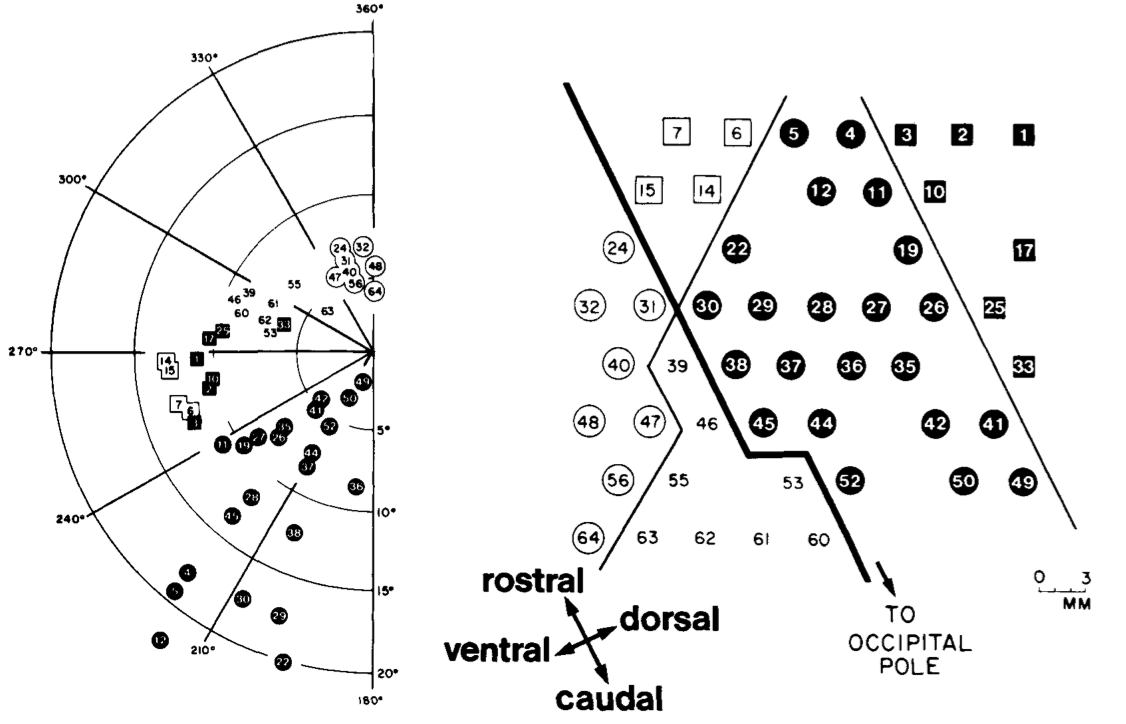
\includegraphics[width=.9\linewidth]{./graphics/litreview/map.png}
\caption{\label{fig:org29f4496}
Spatial distribution of phosphenes mapped to the visual fields (left) in a patient implanted with an early 64-electrode array (right). Figure from Dobelle et al. 1979 \cite{dobelle_mapping_1979}}
\end{figure}

However, while we can very grossly estimate positions of phosphenes in the visual field (especially in relation to the calcarine sulcus, below which phosphenes correspond to superior fields), the distortion of retinotopy on the visual cortex means \emph{precise} mapping is not possible until post-implantation.
In sighted patients, phosphene locations can be mapped with receptive fields in response to visual stimuli, to which they closely correspond. \cite{bosking_saturation_2017,bosking_rules_2018,beauchamp_dynamic_2018}
This is clearly not possible in blind patients, so phosphenes are often mapped by indicating directions or relative positions of pairwise phosphenes. \cite{schmidt_feasibility_1996,beauchamp_dynamic_2018,brindley_sensations_1968,dobelle_mapping_1979}
The implication is that while we can roughly determine the quadrant of a phosphene in the visual field at implantation, we cannot know precisely where it is located until stimulation is trialled.
In addition, sometimes stimulating one electrode produces more than one phosphene, which may be either adjacent or inverted about the horizontal meridian of the visual field. \cite{brindley_sensations_1968,dobelle_phosphenes_1974,schmidt_feasibility_1996}
This is most likely attributable to off-target stimulation of tissue across a sulcus, supported by observations that this phenomena occurs less severely with penetrating microelectrodes (which discharge less than surface electrodes). \cite{dobelle_mapping_1979,schmidt_feasibility_1996}

The space a phosphene occupies in the visual fields varies with eccentricity and stimulation current.
Early evaluations of phosphene size using various objects at arm's length \cite{brindley_sensations_1968,dobelle_phosphenes_1974,dobelle_artificial_2000,dobelle_artificial_1974,schmidt_feasibility_1996} have generally been agreeable with more formal estimates using degrees of visual field. \cite{bak_visual_1990,bosking_saturation_2017,winawer_linking_2016}
Most phosphenes are 1-2\degree  of visual field in diameter and range from 0.1-10\degree  (a "grain of sago" to a coin at arm's length) . \cite{bak_visual_1990,bosking_saturation_2017,brindley_sensations_1968}
The size of phosphenes depends on where they are located in the visual fields; more peripheral phosphenes are larger and reportedly have less distinct borders. \cite{rushton_properties_1978,winawer_linking_2016,bosking_saturation_2017}
The variation of phosphenes with size is consistent with behavioural studies in non-human primary undergoing cortical stimulation \cite{tehovnik_phosphene_2007} and the phenomenon of cortical mangnification, where the central visual field is overproportionately represented on the surface of the brain. \cite{born_cortical_2015}
Phosphenes also appear to increase in size with stimulation amplitude \cite{rushton_properties_1978,winawer_linking_2016,bosking_saturation_2017}, though one early report of microelectrode stimulation also described instances where phosphene size decreased which have not been subsequently reproduced. \cite{schmidt_feasibility_1996}

While circular phosphenes are ubiquitous \cite{brindley_sensations_1968,dobelle_phosphenes_1974,bak_visual_1990,schmidt_feasibility_1996,lee_mapping_2000}, other phosphenes shapes have been reported.
The most consistently reported shape other than circles are elongated elliptical or linear phosphenes oriented in horizontal, oblique or vertical orientations. \cite{brindley_sensations_1968,dobelle_phosphenes_1974,rushton_properties_1978,bak_visual_1990,beauchamp_dynamic_2018}
A few reports identify shapes ranging from triangles and stars, to checkerboards, to face or eye-like hallucinatory sensations. \cite{lee_mapping_2000,murphey_perceiving_2009}
Often, more abstract phosphenes appear on stimulation of later visual areas of the brain, which may not be relevant for prostheses targeting only primary visual cortex. \cite{murphey_perceiving_2009}
While phosphene shapes appear loosely related to the putative role of different brain regions \cite{lee_mapping_2000}, no studies have been able to deliberately control the shape of phosphenes.

Finally, phosphenes have been repeatedly shown to move with eye movements and have been likened to the movement of retinal afterimages. \cite{brindley_sensations_1968,dobelle_artificial_1974,schmidt_feasibility_1996}
It appears the whole map of phosphenes moves as multiple phosphenes maintain their relative positions after movement. \cite{dobelle_artificial_1974,schmidt_feasibility_1996}

\subsection*{Temporal Properties of a Phosphene}
\label{sec:org8ccdd08}

Phosphenes generally appear synchronous with stimulation. \cite{schmidt_feasibility_1996,beauchamp_dynamic_2018}
It is difficult to measure the latency of percepts without also including motor reaction time, but studies comparing phosphene onset reaction times to auditory stimuli suggest that additional latency is minimal. \cite{rushton_properties_1978}
In multiple studies, phosphenes have been sporadically reported to persist for up to 20 minutes after stimulation ceased, particularly after a high-discharge stimulation prior. \cite{brindley_sensations_1968,dobelle_artificial_1974,rushton_properties_1978,schmidt_feasibility_1996}
Perhaps paradoxically, phosphenes purposefully sustained by continuous stimulation demonstrate significant fading in as little as 15 seconds. \cite{dobelle_phosphenes_1974,schmidt_feasibility_1996}
The fading effect of phosphenes is also reflected over separate trials, where phosphenes progressively dim in each subsequent trial (though they "reset" the next day). \cite{schmidt_feasibility_1996}

On a shorter time scale, phosphenes elicited by surface stimulation may also flicker.
The phosphene flicker produced by surface electrodes is fixed, fast, and asynchronous with hardware or physiological pulses. \cite{brindley_sensations_1968,dobelle_artificial_1974,dobelle_phosphenes_1974,rushton_properties_1978,dobelle_artificial_2000}
This differs from the "flicker" produced by two separate successive stimulations, which disappears at stimulation frequencies of approximately 33Hz (though an overlying intrinsic flicker remains). \cite{rushton_properties_1978}
It is unknown whether flicker also occurs in stimulation with microelectrodes; of the few studies of stimlation with penetrating microelectrodes, flicker was not reported.   \cite{bak_visual_1990,schmidt_feasibility_1996}

In summary, we can exert only very limited control over what individual phosphenes look like.
Phosphenes are also highly variable, both between-individuals and between-electrodes.
While there are points of agreement between studies, such as the effect of stimulation current on brightness, other phenomena, such as colour and flickering, remain contentious.
It remains unclear whether these disagreements are due to differences in stimulation parameters, hardware, participants or pathology.

\section*{Phosphenes Produced by Stimulating Multiple Electrodes}
\label{sec:orgbe943f1}

The appearance of images containing multiple phosphenes is fundamental to modern cortical prostheses as very little information can be transmitted through only a single electrode at once. \cite{niketeghad_brain_2019,lewis_restoration_2015}
The intention for cortical prostheses is to produce perceivable \emph{patterns} which can be interpreted.
The eventual hope is to approximate natural images with phosphenes used like pixels of a graphical display.
Early chronic implants operated on this principle, albeit with very low resolution. \cite{dobelle_artificial_2000}

However, the empirical evidence on \emph{what} is perceived when multiple electrodes are stimulated is surprisingly scarce.

At the most simple level, two electrodes which produce individual phosphenes appear to also produce two separate perceivable phosphenes when stimulated simultaneously.  \cite{brindley_sensations_1968,dobelle_phosphenes_1974}
Sometimes, the size of each phosphene decreases compared to individual stimulation, and the distance between phosphenes may increase. \cite{bosking_rules_2018}
When close together, these phosphenes may fuse together into a single percept. \cite{brindley_sensations_1968,dobelle_phosphenes_1974}
However, this is not always the case; in fact, dimmer phosphenes may not be perceived at all \cite{bosking_rules_2018,dobelle_artificial_1974,dobelle_phosphenes_1974}, though there is some evidence that increasing the stimulation amplitude may reintroduce the dimmer percept. \cite{schmidt_feasibility_1996}
As a result, increasing the number of electrodes may not linearly increase the number of perceived phosphenes.

Several studies have characterised greater numbers of simultaneous phosphenes.
Early evidence suggested that four-phosphene patterns (e.g. a square) could be recognised, but not reliably as spurious phosphenes appeared and some expected phosphenes were not perceived. \cite{dobelle_artificial_1974}
Another patient was able to perceive a six-phosphene vertical line. \cite{schmidt_feasibility_1996}
Modern studies, however, have provided conflicting results.
In one study in an epilepsy patient, five electrodes stimulated at once were only able to produce two perceivable phosphenes that was not simply the aggregate of each of the five phosphenes. \cite{beauchamp_dynamic_2018}
In non-human-primates, stimulation of visual cortex simultaneously at two spacially distant points did not sum to an joint signal, further suggesting a separation of processing of simultaneous stimulation. \cite{ghose_strong_2012}

The reasoning behind this difficulty is thought to be because cortical visual prostheses unselectively stimulate local regions of the brain.
In normal primary visual cortex, neurons are typically selectively stimulated by specific image features such as the orientation of lines in the visual fields. \cite{ben-yishai_theory_1995}
When electrodes instead unselectively stimulate neurons, the pattern of neural stimulation is unnatural and later visual areas may not immediately be able to decode the unrecognisable stimulus. \cite{beauchamp_dynamic_2018}

Despite the difficulties of these temporary experiments, chronic studies suggest that patients are able to use this information usefully after a learning period.
There are brief reports of a patient with a chronic implant being able to read phosphene patterns on a 64-electrode implant at 30 letters per minute, similar to Braille \cite{dobelle_braille_1976}
Reports on a different patient from the same group described the ability to recognise symbols and letters at an estimated visual acuity of 20/1200 (seeing at 20 metres what could normally be seen at 1200 metres). \cite{dobelle_artificial_2000}
However, due to the absence of any further chronic studies of implants in blind patients, the upper limit to which people can learn to recognise phosphene patterns is unknown.

Given these limited studies of combinations of phosphenes, there is a tremendous gap between the current knowledge of phosphene patterns and the proposed mechanism of cortical prostheses.
It is entirely unclear whether people can perceive phosphene patterns on the order of tens or hundreds, whether people can learn to perceive these patterns in useful ways, or to what degree these patterns may change.

\section*{Summary of the Perceptual Limitations of Phosphenes}
\label{sec:org0461aeb}

The major issues surrounding the current literature on phosphenes are therefore:

\begin{enumerate}
\item \textbf{There are no modern studies of phosphenes evoked in blind but otherwise-healthy patients, the primary demographic of cortical visual prostheses}.
There are also scant chronic studies, none of which have been conducted with penetrating microeletrodes. \cite{rushton_properties_1978,dobelle_artificial_2000,dobelle_braille_1976}
Emerging clinical trials will help resolve this issue, but until such studies bear fruit, our knowledge on what cortical prosthetic vision looks like may not be readily applicable to new devices.
\item \textbf{Phosphenes are highly variable}.
Almost all features of phosphenes display uncontrollable variability, and the only two properties of phosphenes we have been shown to reliably control are phosphene brightness and size. \cite{rushton_properties_1978}
This variability permeates between electrodes, between patients and between studies.
The heterogeneity, low sample size and skewed populations of the literature have made it difficult to distinguish the root cause of such variation.
\item \textbf{The interpretibility of patterns formed by multiple phosphenes is unclear.}
There is conflict amongst studies on whether multiple phosphenes at once can be integrated simultaneously, or whether people can learn can compensate for initial difficulties with interpreting phosphenes.
\end{enumerate}

As a result, there is considerable uncertainty on exactly what visual sensations modern devices can give to implantees on a case-by-case basis.

\clearpage

\chapter{How can we make what people see most useful?}
\label{sec:org9beda7d}
\label{orgdf1d92a}

Our ability to control the appearance of individual phosphenes and their patterns is clearly limited.
In this section, we briefly review current literature on how images can be represented strategically in phophene space to overcome these limitations.

\section*{The Role of Simulated Prosthetic Vision}
\label{sec:orgea84e6a}

Because of the difficulties of implanting electrode arrays, little research has been conducted on what methods of representing information in phosphene space are most useful \emph{in vivo}.
The only cortical implant which has been connected to a camera in humans was the Dobelle Implant in 2000. \cite{dobelle_artificial_2000}.
The Dobelle Implant used direct image processing techniques fitting of the software capabilities of the time, which essentially downsampled the camera image and directly mapped the brightness to implant electrodes. \cite{dobelle_artificial_2000}.
The group briefly entertained the idea of using edge-detection for more selective stimulation, but no subsequent studies reported the outcomes of this idea.

To allow the testing of new image processing algorithms in the absence of access to real implantees, research in image processing algorithms has largely moved to simulations of prosthetic vision. \cite{chen_simulating_2009-1,chen_simulating_2009}
Simulated prosthetic vision is the primary vehicle through which most new image processing algorithms are tested.
The features of simulated prosthetic vision have been reviewed previously. \cite{chen_simulating_2009-1}
Briefly, camera information is processed and rendered onto a head-mounted or other display as simulated phosphenes.
Typically, these simulated phosphenes are rendered as the most commonly reported percept - white dots with a Gaussian blur filter applied. \cite{chen_simulating_2009-1}
In this way, phosphene "images" are displayed for the user with the aim to approximate the prosthetic vision of an implantee.
Examples of these simulated renders are shown in Figure \ref{fig:org5a51f5c}.

\begin{figure}[htbp]
\centering
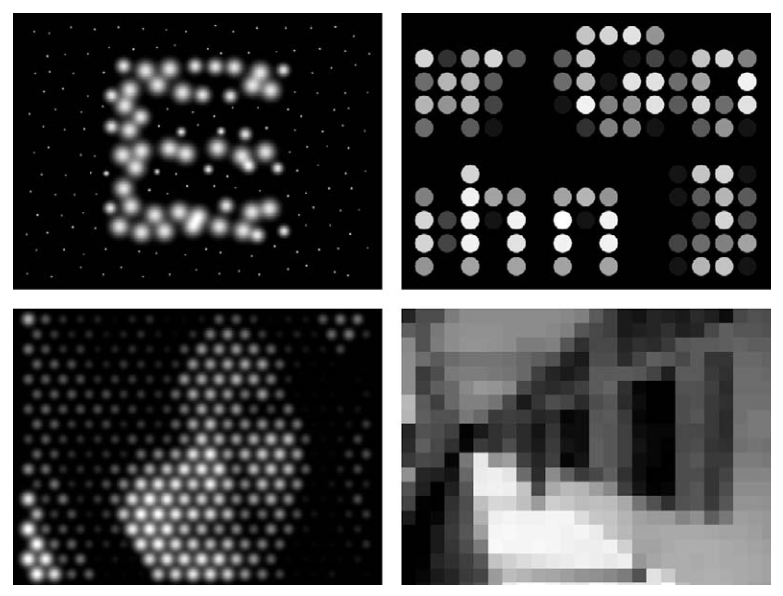
\includegraphics[width=.9\linewidth]{./graphics/litreview/simulated.png}
\caption{\label{fig:org5a51f5c}
Examples of different simulated renders of phosphenes. Figure from Chen et al. 2009. \cite{chen_simulating_2009-1}}
\end{figure}


\section*{A Brief Outline of Current Image Processing Approaches}
\label{sec:org7ef356a}
\subsection*{Direct Methods}
\label{sec:org130efc7}

The prevailing paradigm of image processing for early cortical prostheses was to directly map camera images to a grid of electrodes as though they were superimposed. \cite{schmidt_feasibility_1996,dobelle_artificial_2000}
This produces a phosphene image like a mask full of holes placed on top of the original image.
In this way, prosthetic vision began by attempting to emulate natural vision as closely as possible.

Such an approach may work with a large number of electrodes if all phosphenes could be interpreted correctly as "pixels".
One study estimated that approximately 625 phosphenes would be sufficient to reach a visual acuity of 20/30, suitable for most general tasks \cite{cha_simulation_1992}.

However, there are several issues of direct methods when compared with the perceptual limitations of phosphenes:
Direct methods, by virtue of keeping faithful to the original image, tend to produce simulated phosphene renders with large numbers of "on" phosphenes, particularly in well-lit environments.
As the ability to interpret multiple phosphenes simultaneously is not well established, stimulating many electrodes at once may not produce the expected visual percept.
Because of the high variability of phosphenes, it is also unlikely that the quality and spatial distribution of pixels of a transformed image could be reproduced as faithfully as intended.

Moreover, the quality of these methods very rapidly degrades once resolution drops. \cite{li_image_2018}
No new implants are capable of producing 625 distinct phosphenes. \cite{lewis_restoration_2015}
Without the resolution to support the interpretation of low-level features of directly processed images, images can be uninterpretable.

\subsection*{Edge-Based Methods}
\label{sec:orgd291ca3}

Edge-detection refers to image processing algorithms methods which highlight the edges of objects only. \cite{canny_readings_1987}
Edges require less phosphenes at once and may reduce the amount of redundant information in an image.
This is important when we can consider that the number of perceivable phosphenes may not increase linearly with the number of stimulated electrodes. \cite{bosking_rules_2018}

Edge detectors such as the Canny \cite{canny_readings_1987} edge detector are widely used.
These edge detectors are able to detect fast pixel gradients in images, which typically occur at boundaries.
If additional inputs to the processing algorithm are possible, then more sophisticated techniques can be used.
For example, the use of a range camera or other depth sensing devices can be used to more intelligently find non-background edges. \cite{lui_transformative_2012}
State-of-the-art convolutional neural networks (CNNs) have also been applied to edge detection for prosthetic vision by semantic pixel labelling of images of rooms and determining edges by boundaries between walls. \cite{sanchez-garcia_structural_2018}
An illustration of an edge-detection algorithm combined with a object-filling algorithm is shown in Figure \ref{fig:orgfa3d114}.

\begin{figure}[htbp]
\centering
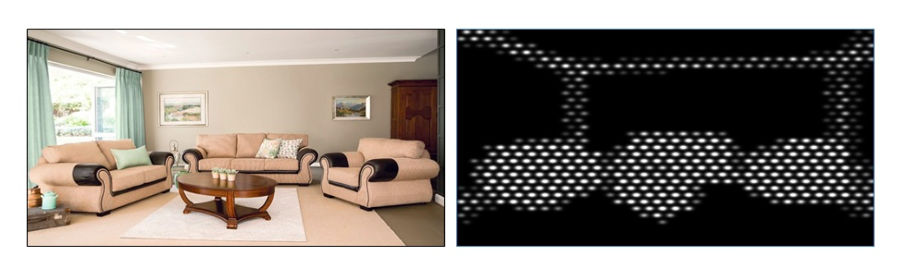
\includegraphics[width=.9\linewidth]{./graphics/litreview/edgeandfill.png}
\caption{\label{fig:orgfa3d114}
An example of an edge-detection algorithm with a CNN-driven object-filling algorithm to render a clean simulated phosphene image. Figure from \cite{sanchez-garcia_structural_2018}}
\end{figure}

The difficulty with edge-based methods is that edges easily degrade when resolution drops, similar to direct methods. \cite{buffoni_image_2005}
One method which aimed to resolve the fragility of edges combined edge-based methods with saliency-based methods to give greater form to objects. \cite{han_object_2015}
Such hybrid methods may be more robust than the use of pure edges when faced with significant downsampling.

\subsection*{Saliency-Based Methods}
\label{sec:org947fef6}

As opposed to naively translating brightness values of camera images to electrode stimulation, saliency-based measures more intelligently identify the semantics of objects in a scene.
Using this semantic structure, the image can be divided or \emph{segmented} into regions of interest which carry a common semantic meaning (e.g. "background" or "foreground"). \cite{pal_review_1993}

With this approach, more deliberate differences between foregound and background can be made as depicted in Figure \ref{fig:org092176d}. \cite{guo_optimization_2018}
When applied to an image classification task, saliency-based methods improved the recognition accuracy of common objects. \cite{han_object_2015,li_image_2018}

Object detection neural networks have also been applied to highlight particular salient features of an image. \cite{mace_simulated_2015}
In these methods, powerful image classification algorithms are able to detect a specified object and solely highlight that object on the simulated phosphene render.
While these methods were constrained to only specific objects, they demonstrate leverage of modern progressions in image processing to intelligently identify objects.

\begin{figure}[htbp]
\centering
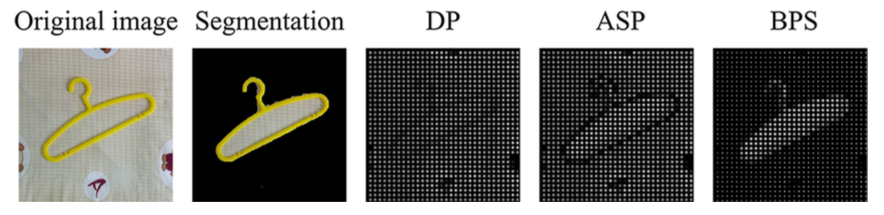
\includegraphics[width=.9\linewidth]{./graphics/litreview/saliency.png}
\caption{\label{fig:org092176d}
An example of a saliency-based algorithm to highlight a region of interest of the image. Figure from \cite{li_image_2018}}
\end{figure}

The methods help highlight what is most likely to be relevant in an image and suppress background, which may otherwise interfere.
However the usefulness of this masking approach is importantly constrained by the implantee's ability to subsequently recognise what is being shown.
While simulations have demonstrated the utility of this approach, the fidelity of the mask form when phosphenes are irregularly shaped and sized is not clear.
While these methods are advantageous compared to direct methods in that irrelevant information may be reduced, it faces the same limitations that low-level forms may be obscured by phosphene distortions.

\subsection*{Transformative Methods}
\label{sec:orga5df359}

Recent advances in machine learning have meant that computers are now reaching human-level abilities for tasks such as image classification using deep learning methods. \cite{rawat_deep_2017,guo_deep_2016}
Because the processor in a cortical visual prosthesis has access to the full camera image (as opposed to the user, who can only see the phosphene version), the processor has more information available to interpret.
Instead of expecting the user to interpret high-level information from degraded phosphene images, some interpretation could be relegated to the computer which can then intelligently re-encode the information in a deliberate manner.

Numerous patents have been filed for such a system. \cite{chichilnisky_eduardo-jose_smart_2018,li_going_2013}
In these systems, important visual cues such as stairs, faces and bank notes are recognised by the computer, which can then remove unnecessary low-level detail and produce compact, abstract images that represent the \emph{concept} of what is seen, not what is actually seen.
For example, faces can be recognised and re-encoded as emoticons which cleanly fit in low-resolution space. \cite{lui_transformative_2012}
An example of this approach is shown in \ref{fig:org39721af}

\begin{figure}[htbp]
\centering
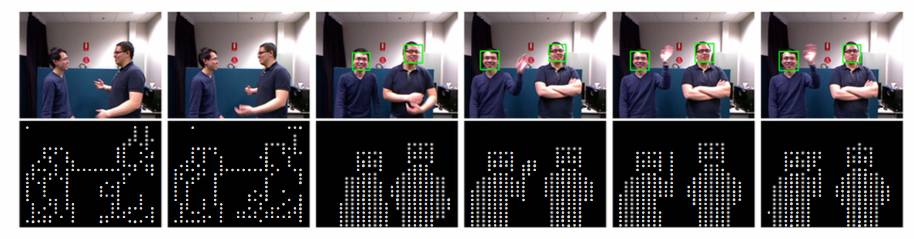
\includegraphics[width=.9\linewidth]{./graphics/litreview/transformative.png}
\caption{\label{fig:org39721af}
An example of a transformative approach to image processing to re-encode information. Figure from \cite{lui_transformative_2012}}
\end{figure}

The chief benefit of such methods is that useful information can be communicated with less phosphenes.
Since many low-level details (e.g. "is this bank note folded at the corner?") are not always relevant, the information burden to the user can be reduced to only what is necessary.

The perceptual issues facing these methods are that these typically rely on producing phosphene images that "mimic" real life (e.g. emoticons, which attempt to mimic faces). \cite{lui_transformative_2012}
However, the perceptual distortions and variability of phosphenes make it unclear whether these mimics could be replicated and thus the ability to specifically evoke these "mimics" \emph{in vivo} with phosphenes is not well established.
What may appear cleanly represented in simulated phosphene space may be heavily distorted and even unrecognisable in real implantee settings.
A potential rebuttal is that as these methods re-encode information at the bequest of the algorithm implementer, they could be optimised on a case-by-case basis for the particular phosphenes an implantee sees.
Individual-level implementations of image processing algorithms are yet to be explored.

\subsection*{Temporal Methods}
\label{sec:org169525b}

Given the challenges already faced by patients when trying to interpret multiple simultaneous phosphenes, some groups have begun to explore non-simultaneous methods of conveying patterned information.
\emph{Dynamic current steering}, where phosphene patterns are "traced" in quick succession rather than presented all at once have shown sigificant benefits for letter recognition tasks. \cite{beauchamp_dynamic_2018,spencer_creating_2018}
Figure \ref{fig:org197f318} illustrates the principle behind this approach.
Patients, without prior training, were able to trace the path of phosphenes and interpret simple letterforms accurately.
Unlike most of these other methods, dynamic current steering \emph{has} been tested \emph{in vivo} in patients with epilepsy with subdural surface electrodes and in fact arose out of perceptual difficulties noted by the investigators. \cite{beauchamp_dynamic_2018}
This highlights one of the issues with simulated prosthetic vision tests; fundamental perceptual differences of electrical neural stimulation may not be discovered and accounted for until tested in real patients.

\begin{figure}[htbp]
\centering
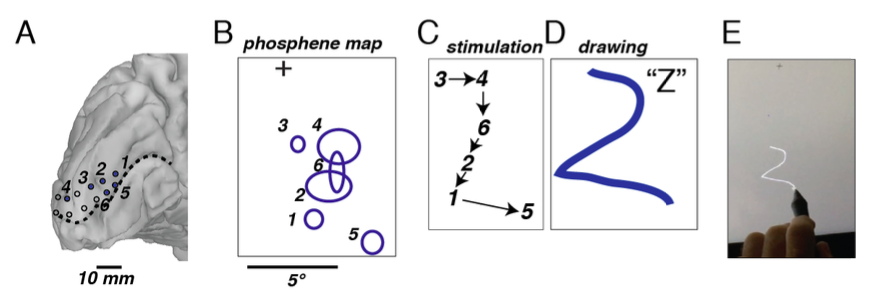
\includegraphics[width=.9\linewidth]{./graphics/litreview/temporal.png}
\caption{\label{fig:org197f318}
An example of a temporal approach to conveying information through phosphenes, where electrodes are stimulated in succession instead of simultaneously. Figure taken from \cite{beauchamp_dynamic_2018}}
\end{figure}

These methods attempt to resolve the issues surrounding interpreting multiple simultaneous phosphenes by tapping into the brain's natural ability to interpret gross motion. \cite{grossman_brain_2002}
While temporal methods may be slower at conveying information per unit time, they have the advantage of not requiring simultaneous presentations of phosphenes, and requiring less current as only a limited number of phosphenes need to be conveyed for a single frame.
It is clear, however, that the difference between temporal methods and form-based methods cannot be assessed in simulated prosthetic vision as the differences between these two methods is based on differences in \emph{in vivo} perception.
More clinical trials are needed to establish whether temporal methods of information transfer as opposed to spatial methods are better suited for cortical prosthetic devices.

\section*{The Limitations of Simulated Prosthetic Vision}
\label{sec:orge284c25}

The crux of many of these methods rests on tests of simulated prosthetic vision, faces significant limitations for generalisability to \emph{in vivo} implants:

\begin{enumerate}
\item \textbf{The possible difficulties \emph{in vivo} of interpreting phosphenes are not accounted for.}
One of the key unknowns in phosphene space are how well the brain can learn to decipher the unselective unnatural stimulation of visual cortex by multiple electrodes simultaneously. \cite{beyeler_learning_2017}
Because our uncertainty in this area relates to the unnatural neural stimulation of the visual cortex, this cannot be assessed in a simulated setting.
When phosphenes are simply shown on a display, a sighted subject naturally is able to process the displayed patterns making full use of the retinal and neural circuity distal to the brain.
This is most certainly not the case for an implantee.
While normal-sighted subjects have often been shown to be able to recognise complex patterns with many simultaneous phosphenes in a simulated setting \cite{chen_simulating_2009}, it is still unclear whether this can be replicated in real implantees.
\item \textbf{Phosphene simulation often does not account for all known properties of phosphenes.}
The properties we have described above are rarely all accounted for.
For example, temporal effects such as fading and accommodation are not implemented in most simulations.
Additionally, most simulations render phosphene images as low-resolution greyscale images with uniform circular \cite{mccarthy_mobility_2014,hu_recognition_2014,sanchez-garcia_structural_2018,li_image_2018} or hexagonal pixels. \cite{chen_effect_2004}, though some studies have also incorporated biologically-based retinotopic distortion. \cite{josh_real-time_2011,josh_psychophysics_2013}
Indeed, many simulated prosthetic vision algorithms approach the problem as chiefly one of low resolution, loss of colour and distortion.
This does not accurately reflect the rich (but uncontrollable) perceptual experiences previously reported by \emph{in vivo} experiments in shape, size, colour or flicker.
\item \textbf{Many simulations use regular and higher-resolution phosphene grids than have previously been achieved.}
Sometimes, psychophysical experiments render on the order of a thousand phosphenes \cite{sanchez-garcia_structural_2018,li_image_2018,guo_optimization_2018}
This far outstrips the number of phosphenes which have been tested simultaneously \emph{in vivo} so far (less than a hundred) \cite{dobelle_artificial_2000}, and also surpasses the estimates of capabilities of modern prostheses. \cite{lewis_restoration_2015}
Ultimately, the ability to reliably evoke many cortical phosphenes regularly and of the calibre of many simulations has not been established.
\item \textbf{Most simulations do not specifically target cortical phosphenes.}
Most advances in image processing methods for simulated prosthetic vision are targeted at retinal prostheses, for which there are already commercially available devices. \cite{stingl_interim_2017,luo_argus_2016,markowitz_rehabilitation_2018}
The lack of distinction between different biological methods of evoking phosphenes in some experiments of simulated prosthetic vision mean results may not be directly translatable.
\end{enumerate}

The implication of these issues is that studies of image processing algorithms in simulated prosthetic vision are not flexible for different phosphene percepts.
The methods we have described are dependent on being able to replicate the simulated renders in \emph{in vivo} implants, but little research has been conducted on this area.
It is unclear how the image processing algorithms produced by studies of simulated prosthetic vision could be made flexible for the variability in phosphenes previously described.

\section*{Future Directions from Advances in Machine Learning}
\label{sec:orga8b551d}

The remaining goal for better addressing the perceptual limitations for phosphenes is to find flexible ways to reconcile image processing algorithms in simulated phosphene space with the wide variability in what phosphenes look like.
Image processing outside of prosthetic vision has experienced a wealth of improvements from advances in machine learning, where computers learn patterns from data without prior knowledge of those patterns. \cite{guo_deep_2016}
Machine learning for image processing is most often applied to the training of \textbf{convolutional neural networks} (CNNs), which are layered architectures of image filters modelled after the function of physiological neurons. \cite{rawat_deep_2017}
CNNs have already discovered widespread use in image recognition tasks \cite{krizhevsky_imagenet_2012}, video recognition tasks \cite{karpathy_large-scale_2014} and style transfer tasks, where images are modified to mimic the style of other images. \cite{gatys_image_2016}

The benefit of CNNs is that they produce image processing algorithms that are trainable from data without requiring explicit programming.
This could be applied to the current gap between simulated prosthetic vision and perceptual limitations of phosphenes.
By training CNNs on task performance data rather than programming algorithms to produce explicit patterns of phosphenes, CNNs could learn to process images in phosphene-agnostic ways.
CNNs could also be tailored for individuals' perceptions of phosphenes, as the dependency of the algorithm shifts towards task performance tests rather than perceptual tests.
This essentially posiions the problem of deriving image processing algorithms from bottom-up (from phosphenes to algorithm) to top-down (from performance to algorithm).

To our knowledge, CNNs have not been applied in this way to derive image processing algorithms for prosthetic vision, and thus research on this topic is scant.
While CNNs and other neural network architectures have been applied to prosthetic vision to construct new algorithms \cite{mace_simulated_2015,ge_spiking_2017,sanchez-garcia_structural_2018}, these have typically been object detection networks involved in segmentation-based processing.
There has also been growing interest in using machine learning recognition algorithms for transformative techniques in prosthetic vision. \cite{chichilnisky_eduardo-jose_smart_2018}
With continuous improvements in the capacity of hardware to support advanced processing \cite{moore_cramming_1998}, it is possible that emergent research in using machine learning to produce flexible, trainable algorithms could improve the utility of a cortical visual prosthesis.

\clearpage

\chapter{Conclusion}
\label{sec:orgf53cf21}

Cortical visual prostheses are a promising enabling technology for the blind.
As the development of these prostheses is still in early stages, it is still not precisely known what type of vision implantees will be able to achieve with a prosthesis.
However, early studies of cortical stimulation seem to suggest that the visual percepts produced will be highly variable and difficult to control.
Whilst there have been many progressions in image processing algorithms in simulated prosthetic vision, the ability of these algorithms to translate to the diverse range of \emph{in vivo} phosphenes is unclear.
This is because many of these algorithms are based on conceptions of the appearance of phosphenes which we do not know if we can replicate, particularly between different people.
There is therefore a gap in the literature between how image processing algorithms could be derived flexibly in a phosphene-agnostic way.
Modern advances in machine learning have shown outstanding achievements of layer image filter architectures, or convolutional neural networks, to learn image processing algorithms from data without explicit programming.
As these methods have not been applied to prosthetic vision before, preliminary studies which assess the feasibility of using machine learning methods to address the perceptual limitations of phosphenes may be greatly informative.

\chapter{Project Motive}
\label{sec:orga129e02}

\section*{Research Questions}
\label{sec:org1046267}

As there are no prior studies applying GANs to simulated prosthetic vision, this project aimed to address the following research questions::

\begin{enumerate}
\item Can GANs be used to train a neural network to produce phosphene patterns representing digits, given different simulated properties of prosthetic vision and, if so, how could this be implemented?
\item Do people find it easier to recognise digits from phosphene patterns derived from training via GANs, compared to a basic comparison (directly masking digits with a phosphene grid)?
\end{enumerate}

\section*{Aims and Hypothesis}
\label{sec:org8b5d0e1}

To address the two research questions, this project aimed to:

\begin{enumerate}
\item Develop a preliminary software implementation of a GAN training architecture for generating phosphene patterns, which could be applied to different phosphene simulations with minimal modification.
\item Experimentally test whether people find it easier to recognise digits from phosphene patterns derived from our prototype training implementation, compared to a basic mask-based comparison.
\end{enumerate}

Aim 2 relies on the implementation produced in Aim 1 and can be hypothesis-tested against the folowing hypothesis:

\begin{enumerate}
\item Sighted participants, under simulated conditions, have a higher overall digit recognition accuracy when viewing phosphene patterns derived from our prototype GAN training architecture, compared to when viewing phosphene patterns produced by basic image processing using masking.
\end{enumerate}

\section*{Rationale}
\label{sec:orgd9b2c59}

While GANs have been applied to image-based tasks in other domains, it is not yet clear how they should be applied to prosthetic vision.
An important difference between GANs in other domains versus prosthetic vision is that typically GANs directly manipulate every pixel in images they generate.
This gives GANs complete control over what its generated images look like and it can optimise the output of each individual pixel.

However, this is not desirable in simulated prosthetic vision where we want to simulate visual experiences which we \emph{cannot} fully control.
GANs must instead be used to generate \emph{instructions} to simulated electrodes, which produce a simulated visual render independent of the GAN based on specified simulation properties.
A useful GAN implementation for simulated prosthetic vision should therefore \emph{not} be based on direct pixel manipulation (as is typically the case).

Aim 1 therefore aims to explore and develop a useful GAN implementation based on separating out a simulated rendering step so that it can be applied to simulated prosthetic vision.
This is the primary contribution of this project.

GANs are designed to minimise the computer's ability to discriminate between generated images and real image samples.
However, computers both find it easy to discriminate features which humans find difficult (e.g. different shades of grey) and find it difficult to discriminate features which humans find easy (e.g. abstract scenes).
As a result, while the generated output may be optimised for a computer, its results may not translate to a human.
Aim 2 is therefore formulated as a preliminary validation measure to test whether the computer's output was human-benefitting.

Aim 2 is \emph{not} intended to provide conclusive or compelling evidence on the usefulness of GANs in general for simulated prosthetic vision.
It is purely intended as a short-term checkpoint on the performance output of the implementation in Aim 1.
It is not expected that this project will produce a necessarily useful software implementation in Aim 1 given its novelty.
The preliminary validation results may instead be used to guide how to better refine the software implementation for future use.

\part{Methods}
\label{sec:org3763a62}
\chapter*{Methodology Overview}
\label{sec:org1f415d4}
This project involved two stages:

\begin{enumerate}
\item Development of a software implementation of a GAN training architecture to derive phosphene patterns of digits, for different types of phosphene simulation properties.
\item Implementation and conduct of a psychophysics experiment to test GAN-trained phosphene patterns (using the implementation developed in the first stage) against basic mask-based controls for a digit recognition task.
\end{enumerate}

\chapter{Development of GAN Training Architecture}
\label{sec:org5a2925c}
\section*{Development Context}
\label{sec:orga3f9e92}

The code required for this project was written by the author using the Python programming language and accompanying software packages.
Where appropriate, some snippets of code have been included below; the remainder of the codebase is too large for inclusion in this manuscript and is therefore hosted and available for perusal at the following GitHub repository (TODO).
All code was developed on a Windows 10 personal computer.
Code was executed both on the development computer (Windows 10) and remotely on the M3 MASSIVE high-performance-computing platform.

\begin{itemize}
\item[{$\square$}] TODO: Host code on GitHub repository (+/- include several files in appendices)
\end{itemize}

\section*{Overview}
\label{sec:org4a5d15d}

A high-level overview of the implemented GAN training architecture is provided in Figure \ref{fig:org6bc4e92}.

\begin{figure}[htbp]
\centering
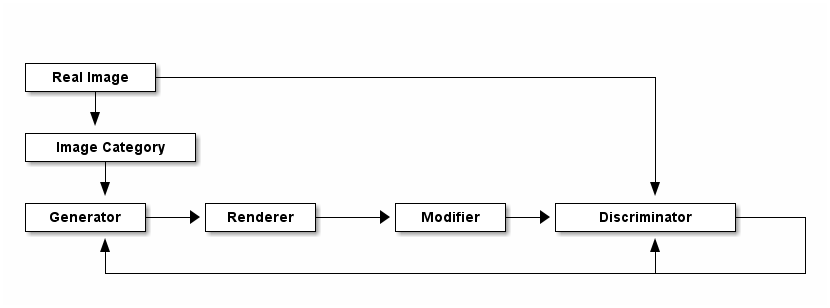
\includegraphics[width=.9\linewidth]{images/methods_training_architecture.png}
\caption{\label{fig:org6bc4e92}
Overview of GAN training architecture implementation.}
\end{figure}

This architecture closely follows classical GAN architectures (explicitly, a conditional GAN architecture), with the addition of the \emph{Renderer} and \emph{Modifier} steps.
The flow of data through the training proceeds as:
\begin{enumerate}
\item A \emph{Renderer} is first chosen for this training run.
The \emph{Renderer} corresponds to a parametric phosphene simulator, which can be altered for different training runs.
\item A real image sample of a digit is taken from a pool of real digits.
\item The image category (in this case, the identity of the digit e.g. a "3") of the image sample is taken from its label.
\item The image category is fed into the \emph{Generator}, which produces a set of instructions - an image \textbf{encoding} - for the \emph{Renderer}.
\item The \emph{Renderer} takes the encoding and simulates it as phosphenes, producing a simulated prosthetic vision image.
\item The \emph{Modifier} takes the simulated prosthetic vision image and modifies it to more closely align it with the domain of the real images.
This is discussed further in the sections below.
\item The \emph{Discriminator} takes both real images, and modified simulated prosthetic images and produces predictions of the digit identity and whether it was real or fake.
The difference of its predictions from the true identities of each image is used to adjust the \emph{Generator} and \emph{Discriminator} to better perform their tasks.
\end{enumerate}

As with classical GAN architectures, the \emph{Generator} and \emph{Discriminator} participate in a zero-sum game where each network has opposing goals; the \emph{Generator} aiming to fool the \emph{Discriminator} into thinking its \emph{Rendered} encodings are real, and the \emph{Discriminator} aiming to identity the \emph{Generator}'s fakes amongst the real samples.

This process is repeated many times to slowly optimise the \emph{Generator} to produce useful encodings that can be fed to the renderer to produce digit-like phosphene patterns.
Each step of this process is discussed in further detail in the sections below.

\section*{Real Images}
\label{sec:org97bb631}

The \emph{Generator} begins training as a naive neural network with no conception of what digits are or what they look like.
In order for the \emph{Discriminator} to train the \emph{Generator} to produce digit-like encodings, the \emph{Discriminator} must be provided samples of what real digits actually look like.

This project used handwritten digit samples from the public MNIST digit dataset. \cite{Lecun1998}
The MNIST digit dataset consists of 60,000 grayscale images stored as 2D pixel arrays with dimensions 27x27 pixels.

The MNIST digits are advantageous because:
\begin{enumerate}
\item It is a publicly-available, comprehensive, labelled, clean, and well-validated dataset (indeed, often the \emph{de facto} dataset for benchmarking machine-learning tasks).
\item Handwritten digits ensure there is sufficient variation within the dataset so that the \emph{Generator} and \emph{Discriminator} are incentivised to learn general features of digits (as opposed to rote-memorising whole digits, as might occur with using digits in a standard font).
\end{enumerate}

Samples of the raw MNIST digit dataset are provided in Figure \ref{fig:org39d60e5}.

\begin{figure}[htbp]
\centering
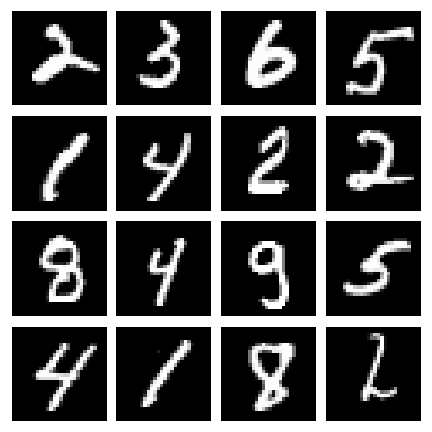
\includegraphics[width=.9\linewidth]{./images/mnist_samples.png}
\caption{\label{fig:org39d60e5}
16 randomly-selected digits from the MNIST handwritten digit dataset.}
\end{figure}

In order for the \emph{Discriminator} to produce useful optimisations, there must be no obvious systematic difference between renders produced by the \emph{Renderer} and the real images.
If such systematic differences were present, the \emph{Discriminator} would have no difficulty discriminating real and generated images and the \emph{Generator}'s output would therefore shift aimlessly as it tries to converge to an impossible goal.

A series of adjustments were therefore performed on the real images to mitigate systematic differences with images achievable by the \emph{Renderer}.
In order to more faithfully simulate a single unilateral cortical prosthetic vision device, we restricted renders to a single half of the visual fields (the right visual field).
We therefore conducted the same adjustment to the MNIST digits by scaling each images' width by half and aligning the result with the right array edge.
Each image's pixel value was also rescaled between -1 and 1 (from 0 to 255) to improve stability of the neural network output and the entire image upscaled to a resolution of 48x48 pixels to equal the pixel resolution of simulated renders.
These adjustments to the real image dataset are illustrated in Figure (TODO).

\begin{itemize}
\item[{$\square$}] TODO: Figure showing adjustments
\end{itemize}

\section*{Image Category}
\label{sec:orgc8a55a9}

The MNIST digit dataset includes a digit label for each handwritten data image in the range 0-9 inclusive.
These image categories are simply encoded as an integer corresponding to their digit label.
As integers (i.e. a numerical datatype), these image categories are suitable for direct input into the \emph{Generator}.

\section*{\emph{Generator}}
\label{sec:orgae2b7e3}

The \emph{Generator} is a neural network which:

\begin{itemize}
\item Takes a single digit in the range 0-9, and
\item Returns instructions to each simulated electrode, as a vector of floating-point numerical values equal in length to the number of electrodes in the simulated prosthesis.
\end{itemize}

There is a notable difference in the \emph{Generator} network described above compared to traditional \emph{Generators} in GANs: the lack of a random seed input.
This was an intentional choice.
The use of a random input seed into \emph{Generator} networks in GAN architectures allows it to output multi-modal images - i.e. images which are similarly realistic, but possess slight image variations.
This is often desirable, where we want GANs to produce many different novel images instead of just one.

However, for use in simulated prosthetic vision, multi-modal output is a low priority.
Firstly, the ability to incorporate multi-modality into a \emph{Generator} which does \emph{not} have direct access to its final render is not clear.
Secondly, it may actually be desirable to limit the output to one "good" phosphene pattern per digit; in practice, subjects are likely to find it easier to learn one phosphene pattern per digit only rather than having to deal with many "similar" patterns with extra variable features.

Because this is the first attempt at developing a GAN for our purpose, it is unknown what neural network architecture is best suited for this task.
Our task consists of a simple mapping between 10 image categories (digit identities) to deterministic vectors as we purposefully removed the usual random seed input.
We therefore used a neural network with a minimal number of hidden layers to reduce training times, depicted in Figure (TODO).

The \emph{Generator} network consisted of:
\begin{enumerate}
\item An \emph{input} layer, containing a single neuron taking a digit from 0-9 as input.
\item An \emph{embedding} layer, which maps the single categorical digit class into a 10-element continuous vector.
\item A \emph{batch normalization} layer, which applies a normalisation for each mini-batch before feeding into the next layer.
\item A \emph{leaky ReLU} layer, which applies a rectifier activation function to dampen negative values.
\item A \emph{dense} layer, which outputs a vector of simulated electrode instructions for a specified number of electrodes.
\item A \emph{sigmoid} layer, which applies a sigmoid activation function to constrain all output values between 0 and 1.
\end{enumerate}

My passing an image category (digit 0-9) into the \emph{Generator} as input, the \emph{Generator} therefore outputs a vector of simulated electrode instructions according to the specified number of electrodes.
The simulated electrode instructions take the form of a vector of floating-point numbers between 0 and 1 inclusive, with the number of elements equalling the number of electrodes.
Each floating-point number indicates the "brightness" at which an electrode should be activated to represent a particular image category (digit).
Notably, there is no information encoded about what electrode actually \emph{does}, nor where it is located; the \emph{Generator} network is effectively blind to these elements of the simulation.

\begin{enumerate}
\item[{$\square$}] TODO: Graphical depiction of the encoder network
\end{enumerate}

\section*{Renderer}
\label{sec:org704c5ae}

The \emph{Renderer} is a custom simulation of prosthetic vision, which takes instructions for each "electrode" as input, and outputs the simulated render as a grayscale image.
The \emph{Renderer} is a simulated stand-in for real implantees and their perception of vision through a CVP.

The \emph{Renderer} is essentially a 3D volume of pre-rendered 2D grayscale image slices, each slice corresponding to the visual percept of a single electrode.
These pre-rendered grayscale slices allow each electrode to produce a distinct, unique percept; for example, one electrode in the \emph{Renderer} may produce a small phosphene located near the center of vision, while another may produce a much larger phosphene in the peripheries.
When an instruction for each electrode is supplied, each slice in the 3D volume is weighted according to its value.
The slices are then aggregated together by summing along the long axis, and clipping values between 0 and 1 to produce a final grayscale render.
The final render is then rescaled between -1 and 1 before being supplied to the discriminator.
This process is visualised in Figure (TODO).

\begin{itemize}
\item[{$\square$}] TODO: Graphic visualisation of the renderer
\end{itemize}

Because the \emph{Renderer} base is a 3D volume of pre-rendered slices, different subjects can be simulated by using different pre-rendered volumes without requiring changes to the rendering process.
In addition, the use of pre-rendered slices makes training much more efficient, as creating the render consists merely of bulk matrix operations which are easily vectorisable.

In order to generate test grids for use with training, two different means of generating pre-rendered slices were implemented:
\begin{enumerate}
\item Cartesian-spaced phosphenes, which maps electrodes to positions in a regular Cartesian plane and assigns the same size and strength to each phosphene.
This was chosen as a basic control as this grid essentially approximates a normal (albeit low-resolution) pixel image.
\item Polar-spaced phosphenes, which maps electrodes to positions in a regular Polar grid and assigns to each phosphene a size corresponding to its location, as given by the equation \(log(k \times (x^2 + y^2) + a)\) for parametrically-set values \(k\) and \(a\).
This was chosen to more closely reflect the visual qualities of phosphenes known to appear to subjects from experimental trials of cortical stimulation.
\end{enumerate}

For each of the two implementations above, two optional flags were also added:
\begin{enumerate}
\item A randomising flag, which produces phosphenes at random locations instead of along a regular Cartesian or Polar grid.
\item A half-flag, which constrains phosphenes to appear only in a single half of the visual fields (simulating a single implant, inserted into only one hemisphere of the brain).
\end{enumerate}

The \emph{Renderer} can theoretically simulate any number of phosphenes, but for our purposes, we focused on phosphene grids containing 64 phosphenes only.
This reflects a highly conservative estimate of the number of useful electrodes achievable by first-generation CVPs.


These grids are illustrated in Figure (TODO).
\begin{itemize}
\item[{$\square$}] Graphic visualisation of layouts of the grids described in this step!
\end{itemize}

\section*{Modifier}
\label{sec:orgcb54eaa}

In order for GANs to work effectively for the next step (feeding into the \emph{Discriminator}), the generated fake renders must have the capability of looking as close to the real images as possible.
Because the generated renders necessarily create simulated phosphenes, there would usually be no chance of the renders actually looking like digits unless the rendering resolution (i.e. number of phosphenes) was fairly high (at least 27x27 pixels, the original MNIST digit resolution).
To resolve this problem, a \emph{Modifier} network can be added in order to bring the domain of the generated renders closer to the domain of real handwritten digit images to simulate basic "inference" that humans might make.
This amounts to simple "hole-filling" for most purposes - i.e. connecting spaces between phosphenes, as a human might be able to do, and outputting a new "inferred" image.
In this sense, the \emph{Modifier} allows the computer to simulate the sort of inference a person might be able to make from simple phosphene dots into more cohesive outlines and forms.

For this project, the \emph{Modifier} consisted of a simple style-transfer GAN which mapped between phosphene images and "filled" forms.
Style-transfer GANs are well-studied architectures, and the architecture of the \emph{Modifier} closely followed a basic style-transfer GAN architecture comprising:
\begin{enumerate}
\item An \emph{input} layer, taking the entire 2D grayscale render image (reshaped as a 3D slice with a depth of 1).
\item Multiple \emph{2D convolutional} layers (48, 96, 128 and 128 filters), each followed by a \emph{batch normalization} and a \emph{leaky ReLU} activation layer, which progressively downsample the image into extracted features.
\item Two \emph{2D deconvolutional} layers (48 and 1 filter/s), which progressively upsample the extracted features into a new modified image render.
The last layer is passed through a \(tanh\) activation function to remap the output between -1 and 1, as in the original render.
\end{enumerate}
This process is illustrated in Figure (TODO).

In order to train the \emph{Modifier}, MNIST digits were passed under 4800 random polar grids of 64 phosphenes with a simple masking operation to generate pairs of phosphene images real digit images.
These phosphene-real pairs were used to train the weights of the \emph{Modifier} network.
Once the \emph{Modifier} was trained, its weights were saved and frozen for subsequent use as a simple phoshene-to-forms image processor.
Examples of the style transfer output of the trained \emph{Modifier} is shown in Figure (TODO).

\begin{itemize}
\item[{$\square$}] TODO: Reference style-transfer GANs either here or in the Background section.
\item[{$\square$}] Modifier network figures
\end{itemize}

\section*{Discriminator}
\label{sec:org4755bb4}

The \emph{Discriminator} is the final major processing step of the GAN training architecture, and the major element involved in actually training the \emph{Generator}.
The \emph{Discriminator} takes a modified rendered grayscale image, and outputs an 11-element vector of probabilities.
The first ten elements correspond to the probability the \emph{Discriminator} believes the input image is a 0, 1, 2 etc.
The final element corresponds to the probability the \emph{Discriminator} believes that the input image is not a digit at all, and is instead "garbage."
The \emph{DIscriminator} is therefore a classifier which classifies images as either belonging to one of 10 digit classifications, or as being garbage instead.

The \emph{Discriminator} itself is a convolutional neural network with a relatively small number of layers. It comprises:
\begin{enumerate}
\item An \emph{input} layer, taking the 2D grayscale modified render image (reshaped as a 3D slice with a depth of 1).
\item Two \emph{2D convolutional} layers (64 and 128 filters), each followed by a \emph{leaky ReLU} activation function and a 25\% \emph{dropout} layer (randomly discarding 25\% of prior inputs, to protect against overfitting)
\item A \emph{flatten} and a \emph{dense} layer, to output an 11-element vector, which is then passed through a \emph{softmax} activation function to ensure all probabilities add to 1.
\end{enumerate}
This process is illustrated in Figure (TODO).

\begin{itemize}
\item[{$\square$}] TODO: Discriminator network figure.
\end{itemize}

The 11-element vector of probabilities output by the \emph{Discriminator} is then used to train the \emph{Generator} and \emph{Discriminator} itself through their respective loss functions.

\section*{Loss Functions and Training}
\label{sec:org99a8998}

Once an image, generated or real, has passed through to the \emph{Discriminator} to output probabilities, these probabilities can then be used as the basis for adjusting the \emph{Generator} and \emph{Discriminator} to optimise them toward their respective goals.
This is the foundational basis of any GAN training architecture.

The \emph{Generator}'s goal is to have the modified renders produced from its encodings look as indistinguishable from real digits as possible.
When its modified renders are passed through the \emph{Discriminator}, it should therefore be optimised to produce a probability of 1 corresponding to the original \emph{Generator}'s digit class input and a 0 for every other possibility.
The \emph{loss} of the \emph{Generator} is given by the categorical cross-entropy between a one-hot vector corresponding to the original image class input, and the \emph{Discriminator}'s predicted output.

The \emph{Discriminator}'s goal is to correctly classify real handwritten digits into their respective digit, as well as to correctly identify the modified renders produced by the \emph{Generator} as "garbage".
The \emph{loss} of the \emph{Discriminator} is therefore given by the sum of categorical cross-entropies between:
\begin{enumerate}
\item A one-hot vector corresponding to the real digit class of real images, and the predicted output of real images, and:
\item A one-hot vector corresponding to the "garbage" class, and the predicted output of images from modifier renders produced by the \emph{Generator}.
\end{enumerate}

These two losses are backpropagated through the network for each image sample and the weights within the \emph{Generator} and \emph{Discriminator} networks are updated according to their respective gradients over their loss function.
For this project, the optimiser for gradient descent used was the Adam optimiser with a learning rate between 0.0001 and 0.01.

\section*{Performing Training}
\label{sec:orgbe6c42e}

Training was performed in batches of 500 MNIST images, over all 60,000 images for up to 30 or 40 epochs.
All training was performed on the M3 MASSIVE high-performance-computing service, and required approximately 10 hours to complete training for a single specified grid.
The weights of the \emph{Generator} and intermediate phosphene render results were saved after each epoch to permit early stopping and reuse of any epochs renders.
Overall, the training was conducted on over 100 different grids during development; 11 of which were randomly chosen for primarily validation in the psychophysics experiment.
Qualitative results of training were evaluated to guide development at multiple stages during the development process.

\chapter{Psychophysics Experiment}
\label{sec:org2be8d7c}
\section*{Development}
\label{sec:org7698bc0}

A psychophysics experiment was developed in order to perform preliminary validation of the GAN prototype discussed prior.
Ethics approval was obtained prior from the Monash University Human Research Ethics Committee to conduct prosthetic vision simulations in normal-sighted indiiduals for the development of a bionic eye (MUHREC Project Number 12525).
The psychophysics experiment was coded by the author using the Python programming language and the Psychopy psychophysics software package, and is included in the Appendix.

\section*{Recruitment}
\label{sec:org531adf6}

11 participants (9 male, 2 female; ages 21-40) with normal or corrected-to-normal vision were recruited from students and staff at Monash University on a volunteer basis.
Participants were briefed on the purpose and conduct of the experiment and signed a consent form for the experiment.

\section*{Setting}
\label{sec:org84c2857}

Psychophysics experiments were held in a single darkened room at Monash University for all participants.
The room contained a table, a chair, a computer, and a chin-rest mounted on the table.
Other items, including office stationery and books, were present in the room but were not significant for the experiment and not interacted with by participants.
During the experiment, the lights were switched off, the blinds were shut, the door closed and the participant instructed to silence their mobile device, leaving the computer monitor as the only major source of light.
The computer monitor's brighness and contrast were kept the same for all participants.
Participants were allowed to adjust the height of the chair, and vertical height of the chin-rest (but not the horizontal distance from the monitor) as comfortable.
All participants used the same pair of headphones, sanitised between each use, and were allowed to adjust the volume of the headphones as comfortable for their hearing level.

\begin{itemize}
\item[{$\square$}] TODO: photograph of setup?
\end{itemize}

\section*{Conduct}
\label{sec:org3ee3810}

Prior to the psychophysics experiment commencement, a random grid was allocated to each participant.
The experiment consisted of a single approximately one-hour session for each participant.
At the start of the experiment, the participant was asked to sit on a chair in front of a computer screen.
The participant was then asked to rest their chin in a chin rest approximately an arms length away from the computer screen.
The horizontal distance between the chin rest and the computer screen was the same for each participant; participants were allowed to adjust the vertical height of the chinrest within a range of several centimetres to suit their sitting height.
The participant was then given a pair of headphones to wear, and the volume was adjusted for the participant's comfort.
The experimental trial blocks, beginning with an example block, were then commenced.

\subsection*{Trials and Trial Blocks}
\label{sec:orge1827ea}

A \emph{trial block} for this experiment consisted of an uninterrupted set of classification trials, interspersed with grey screens which participants were instructed they could use to take a short pause.
A \emph{trial} for this experiment consisted of an uninterrupted set of phosphene-represented digit \emph{cues} which the participant was asked to identify.
A \emph{cue} for this experiment consisted of a single black screen with a phosphene pattern located in center.
A \emph{condition} for this experiment consisted of either the control condition (a brightness-based mask over phosphenes) or the test condition (the trained \emph{Generator} for the grid allocated to the participant).

Each experimental trial block consisted of 12 trials; each trial consisted of 20 phosphene representations of digits which a participant was asked to classify.
At the start of a trial, the participant would be shown a grey progress screen, instructing them to press any key to continue.
At a keypress, the participant would be shown the first cue, and the program would await a digit keypress from the participant.
When the participant pressed a digit, they would immediately hear audio feedback simultaneously playing a tone indicating if they were correct (high) or incorrect (low), and a voice telling them what the true digit was.
The next cue would then immediately be shown, and the program would await the next digit keypress.
This would repeat 20 times.
At the conclusion of a trial, another grey progress screen would be shown, and the trial process would again repeat.
At the conclusion of a trial block, the participant would be given a short break before the next trial block was begun.

4 participants conducted 2 trials blocks; one for each condition, one after the other.
5 participants conducted 4 trials blocks; two for each condition, interleaved.
The condition participants started with was balanced between both conditions for both scenarios above.

Prior to the commencement of the trial blocks, the participant was given an example trial block to familiarise themself with the procedure of the experiment.
The example trial block consisted of an identical format to the trial blocks above, but contained only 2 trials of 10 digits each.

\begin{itemize}
\item[{$\square$}] TODO - needs more detail, but will come back to this.
\end{itemize}

\section*{Analysis}
\label{sec:orgc26c1a2}

All 11 participants' data were included for analysis.

To statistically address the second aim of this project and its corresponding hypothesis, the classification data was modelled using a logistic regression model, including the effects of:
\begin{itemize}
\item Condition, the primary variable of interest.
\item Cue, trial and trial block and their corresponding interaction effects, which we expected to reflect a training effect.
\item Digit class, which may reflect intrinsic differences between digits' abilities to be represented in arbitrary grids.
\item Participant, which was expected to reflect inter-individual variation.
\end{itemize}

\part{Results}
\label{sec:orgd1cb1c9}

\chapter*{Results Overview}
\label{sec:org8c640af}
The results are divided into:

\begin{enumerate}
\item Training results, showing qualitative phosphene patterns and training statistics of digit encoders produced by training, and
\item Experimental results, derived from participants' performance during the psychophysics experiment described in the previous section.
\end{enumerate}

\chapter{Training Results}
\label{sec:orga15b6d9}

The GAN training architecture described in Section <> was tested on a large variety of phosphene grids varying in phosphene location, sizing, regularity and resolution.
We were successful in applying the training process to different types of phosphene grids, which varied primarily in spatial distribution, phosphene size and phosphene resolution.
We have selected a representative sample of different simulated grid properties to highlight several general features of the training results.
The output here is appraised qualitatively for a broad range of grids, with statistical validation done for a small samples of low-resolution grids in the following section.
A number of additional figures are included in the Appendix as supplementary material.

\section*{Variation over Epochs}
\label{sec:orga9f1f91}

Phosphene patterns initially improved with epochs, but drifted away from recognisable patterns as the number of epochs increased further.
This effect permeated all runs of the training architecture for every grid, and the epoch at which digits appeared "best" varied considerably.
Figure \ref{fig:org3d31b05} demonstrates the evolution of the generated phosphene pattern for the digit 4 for a regular cartesian grid of 576 phosphenes.
Although the phosphene pattern approaches several different depictions of a 4 at epochs 6, epoch 20 and epoch 39, it does not stabilise at a particular point but continues to attempt to reconfigure itself.

\begin{figure}[htbp]
\centering
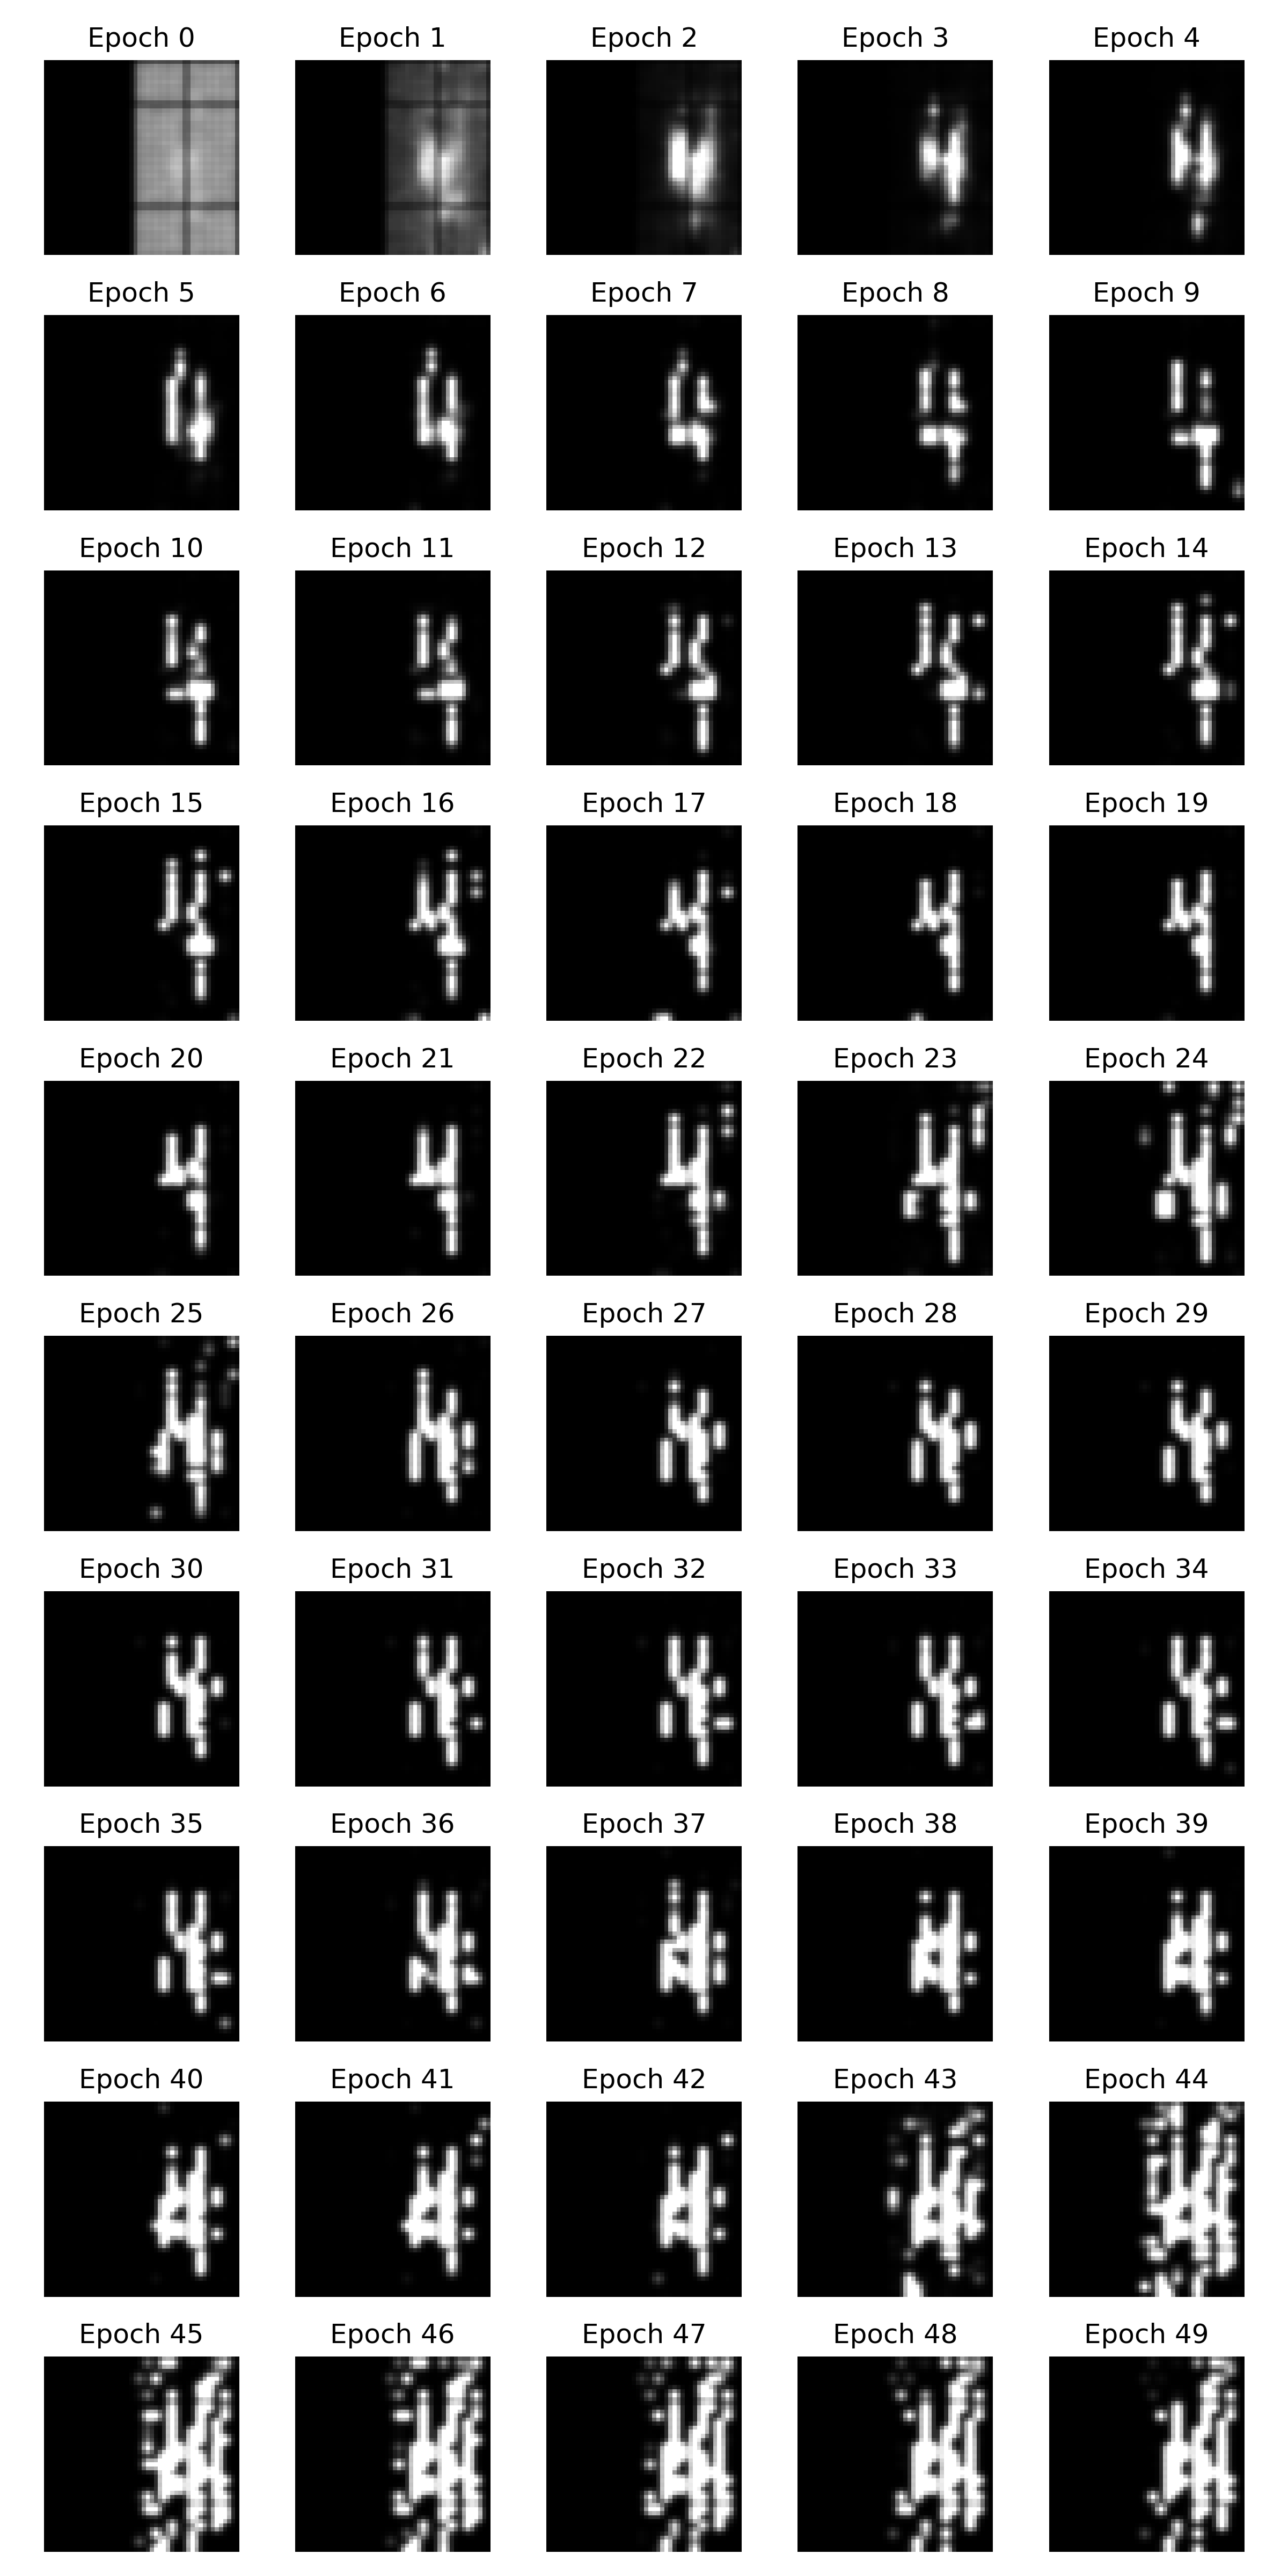
\includegraphics[width=.9\linewidth]{./images/results_over_epochs_576.png}
\caption{\label{fig:org3d31b05}
Phosphene patterns generated for the digit 4 for a regular cartesian grid of 576 phosphenes. The digit form approaches a recognisable digit 4 until approximately epoch 20, before the subsequently drifting away.}
\end{figure}

\section*{Variation over Resolution}
\label{sec:orgc6ded03}

In general, phosphene forms more closely resembled digits at higher phosphene resolutions.
At the lowest resolution tested (64 phosphenes), phosphenes ceased to resemble digits even for the most simple grid, the regular Cartesian grid.
The phosphene patterns generated for a regular Cartesian grid of 64, 144 and 576 phosphenes at 2, 4 and 8 epochs for the digit 0 is shown in Figure \ref{fig:org31a71ad}.

\begin{figure}[htbp]
\centering
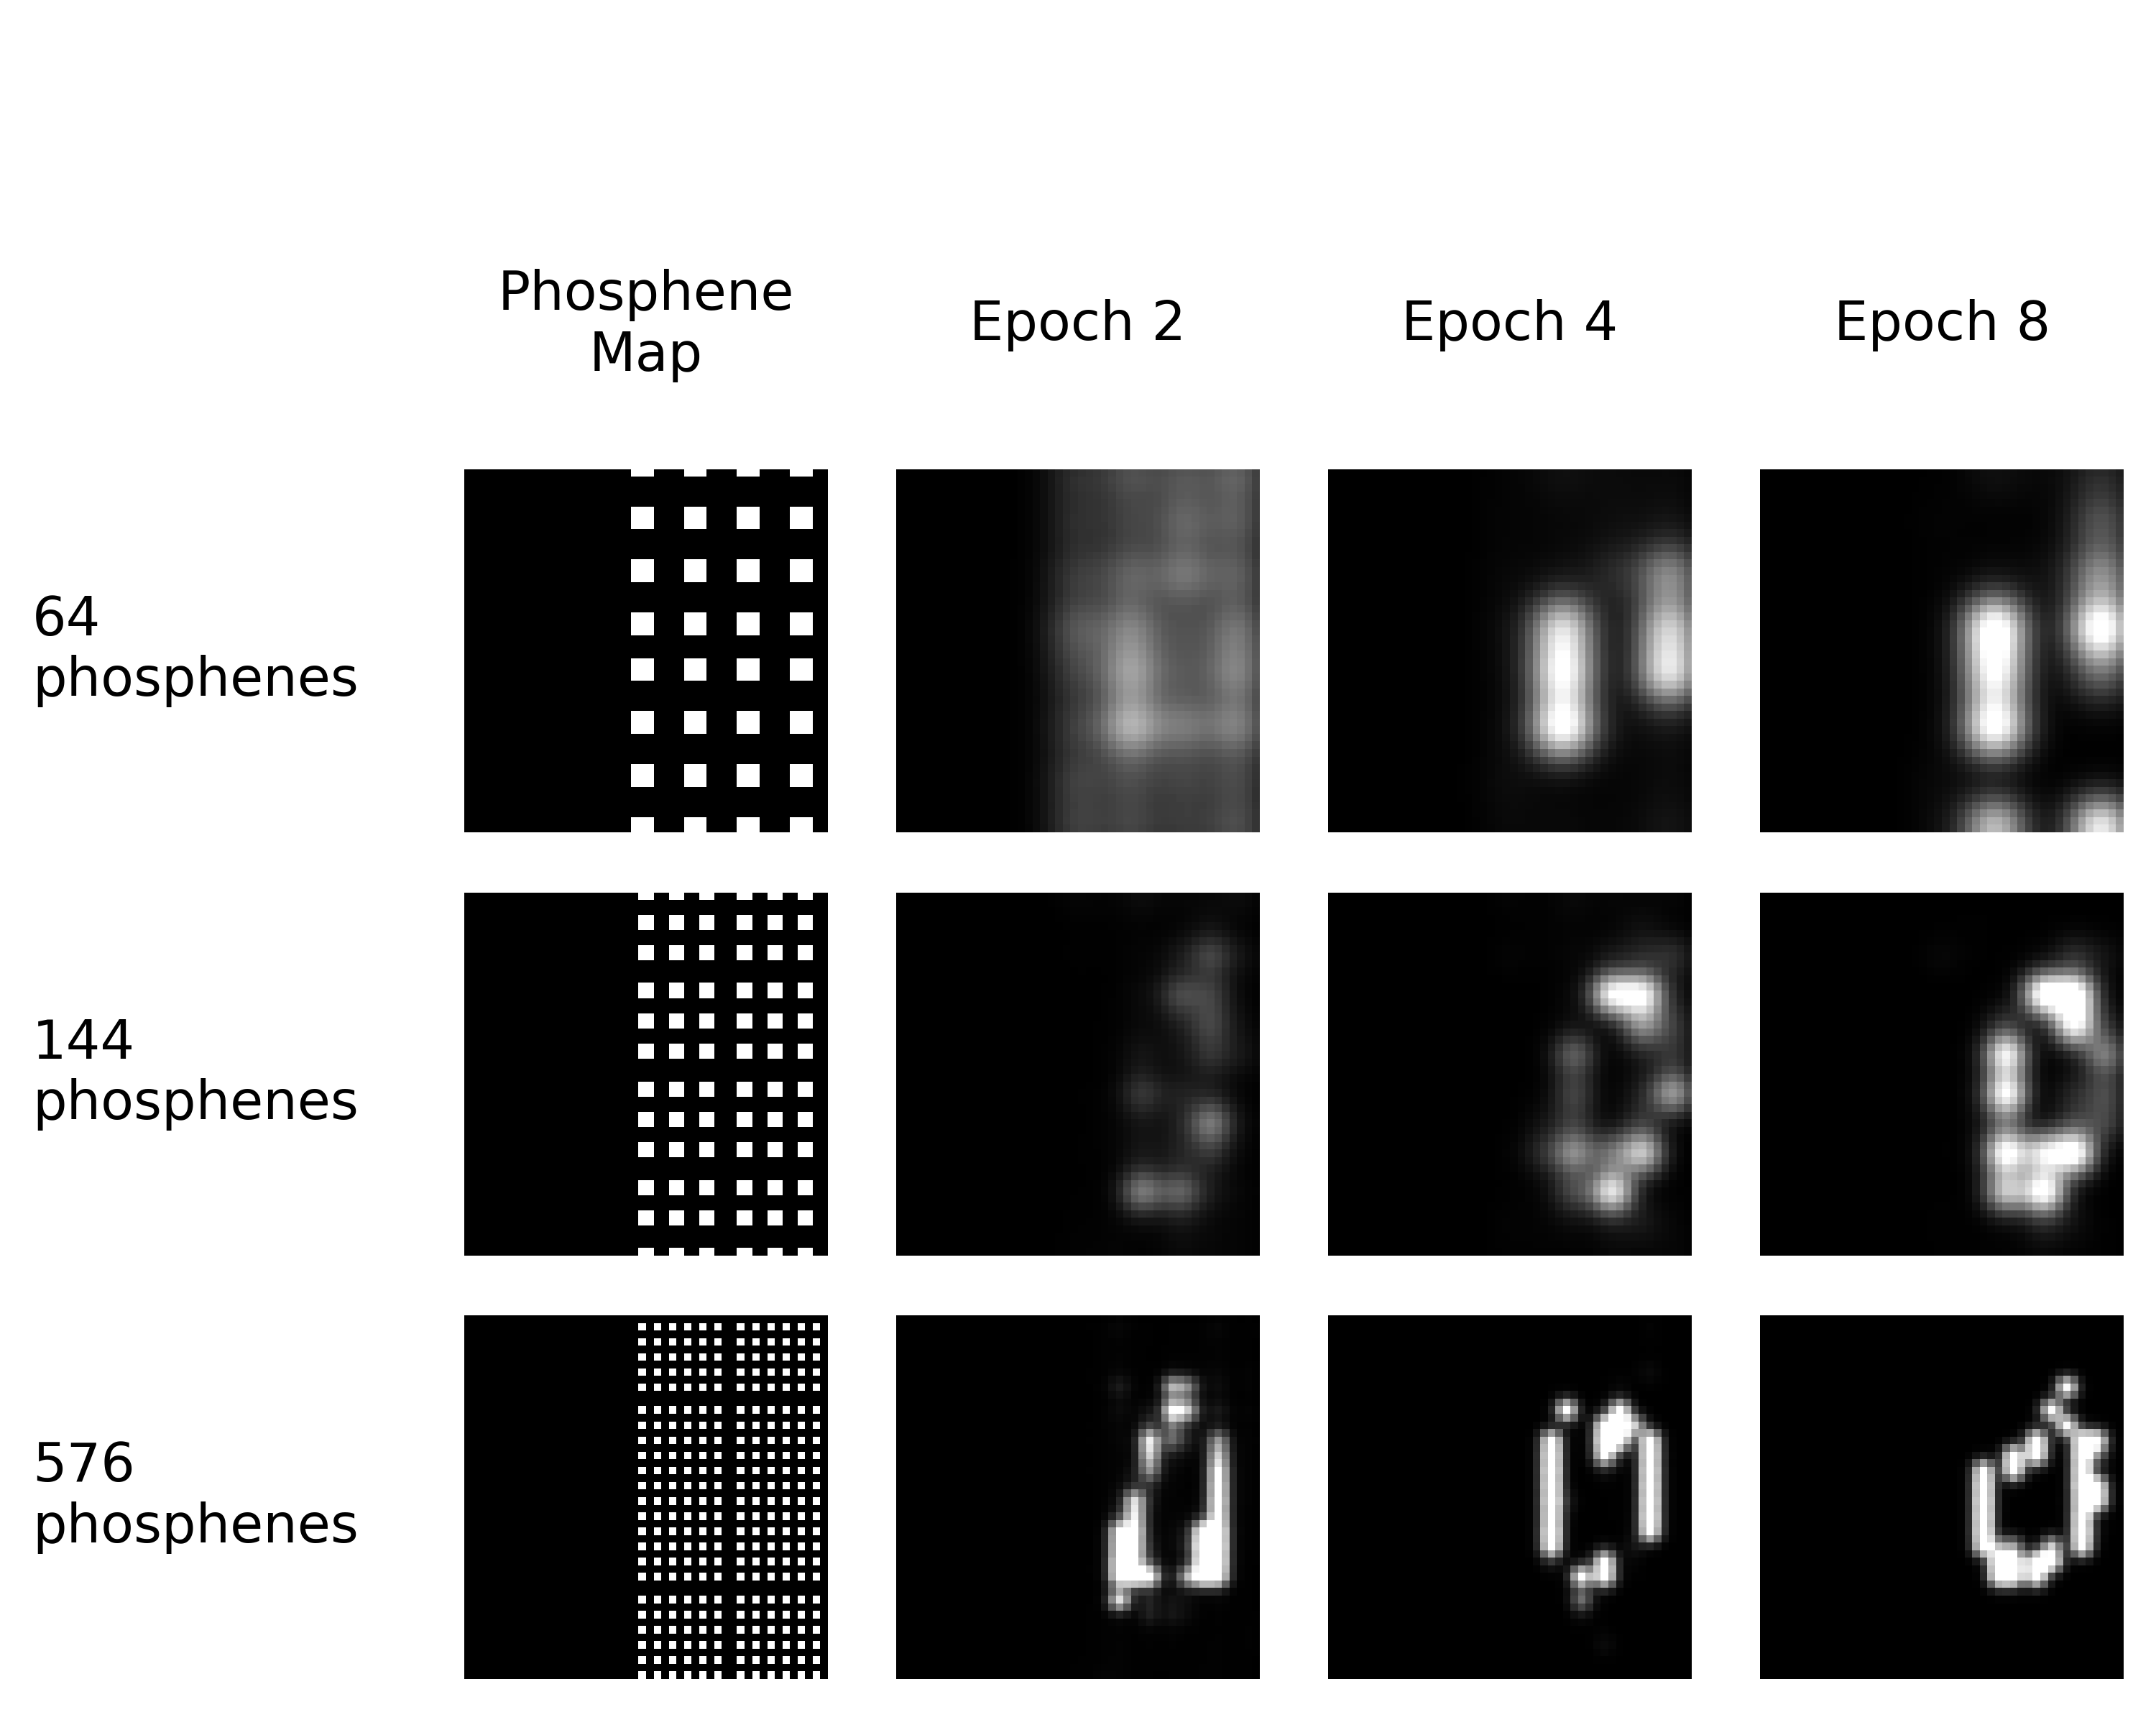
\includegraphics[width=.9\linewidth]{./images/results_different_resolution.png}
\caption{\label{fig:org31a71ad}
Phosphene patterns generated for different phosphene resolutions of a regular Cartesian grid for the digit 0. The first column shows the phosphene locations and relative sizes; the second, third and fourth columns show the simulated patterns at the 2nd, 4th and 8th epoch respectively.}
\end{figure}

\section*{Variation over Grid Arrangements}
\label{sec:org71521d7}

Phosphene patterns were successfully generated for both cartesian and polar grids with regularly and randomly spaced phoshenes.
However, the appearance of these phosphene patterns were often non-optimal at high-resolutions, and non-recognisable at low-resolutions.
Figure \ref{fig:org2a4eb81} shows the generated phosphene patterns for a grid of 576 phosphenes at 10, 20 ad 30 epochs for the digit 6.
Note that the polar grids have considerably larger phosphenes in general (particularly at the peripheries), leading to greater difficulty for the training architecture in producing \emph{any} recognisable forms.

\begin{figure}[htbp]
\centering
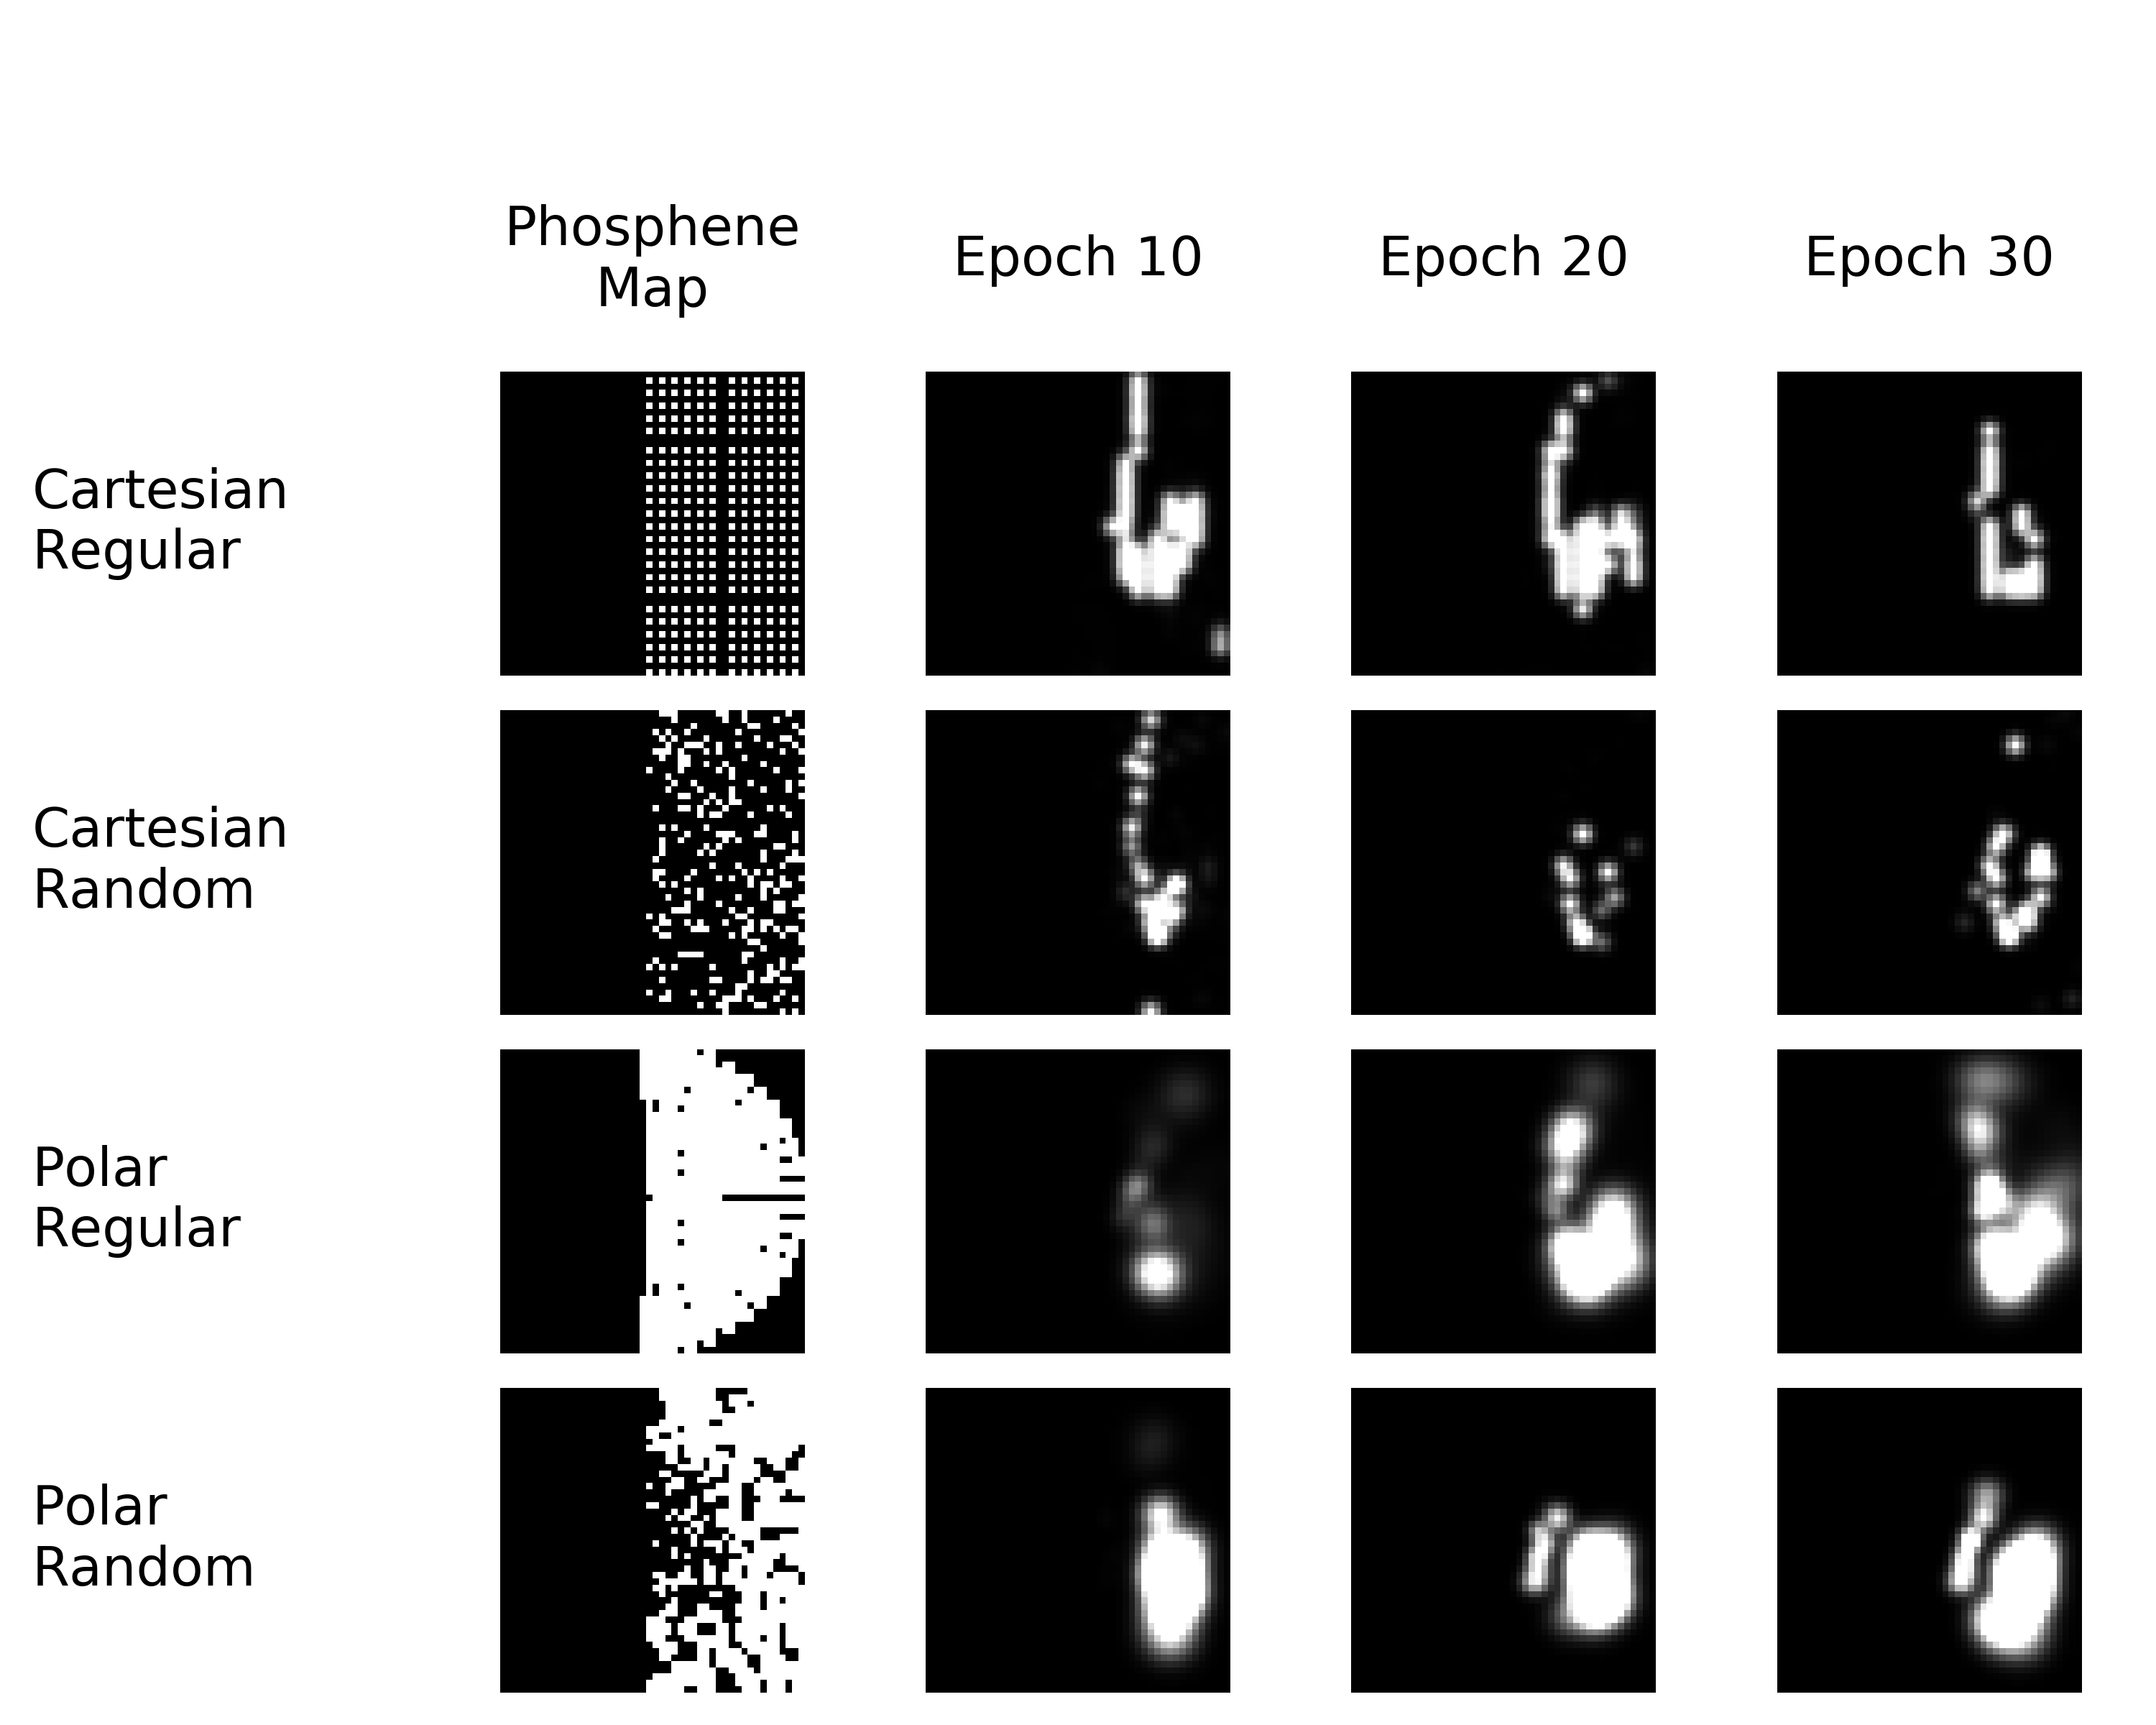
\includegraphics[width=.9\linewidth]{./images/results_different_grids_576.png}
\caption{\label{fig:org2a4eb81}
Phosphene patterns generated for the digit 6 for 4 different grid arrangements with 576 phosphenes at 10, 20 and 30 epochs with the base phosphene map on the left for comparison.}
\end{figure}

\section*{Variation over Digits}
\label{sec:org2558132}

The ability to generate phosphene patterns resembling digits varied dramatically for different resolutions and arrangements of grids.
Figure \ref{fig:org0ca5879} shows the generated phosphene patterns at the 16th epoch for a regular cartesian grid of 576 phosphenes, the highest resolution and simplest arrangement tested.
Phosphene patterns at this stage were recognisable, though there are notable imperfections such as interrupted lines.

\begin{figure}[htbp]
\centering
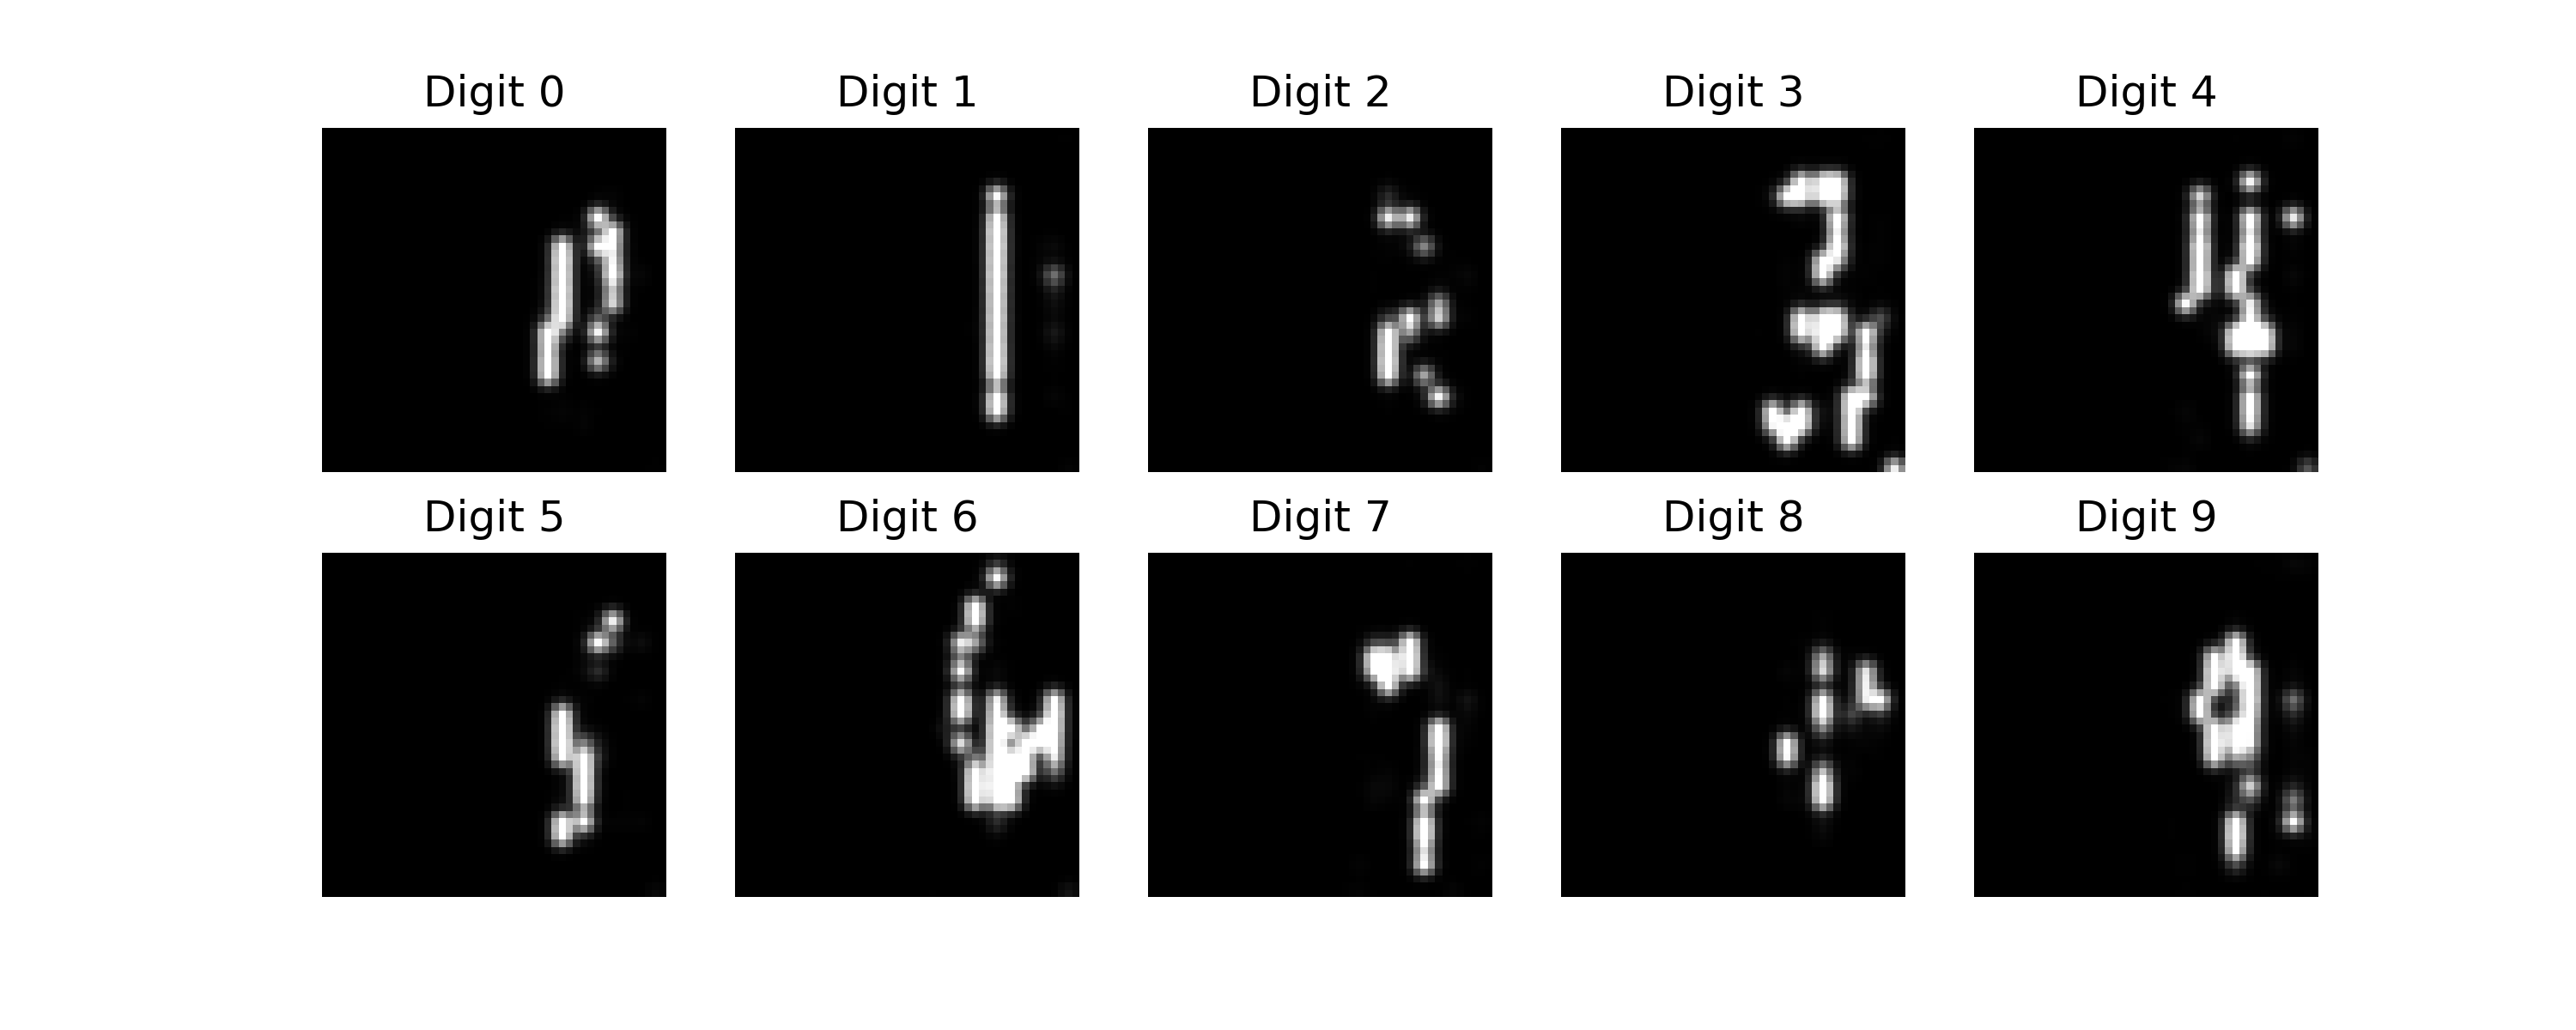
\includegraphics[width=.9\linewidth]{./images/results_over_digits_576.png}
\caption{\label{fig:org0ca5879}
Phosphene patterns generated for each digit 0-9 for a regular cartesian grid of 576 phosphenes at the 16th epoch.}
\end{figure}

\chapter{Experimental Results}
\label{sec:org6986c62}

\section*{Grid Selection}
\label{sec:orgbe17f33}

While the most recognisable phosphene patterns were produced using regular cartesian grids at higher resolution of 576 phosphenes, these simulations are not the primary area of interest for simulated prosthetic vision where grids are irregular and expected to be much lower resolution.
We therefore selected the lowest resolution grids (64 phosphenes) with randomly-arranged polar phosphenes which best reflected the current reality of CVP capabilities.
Due to time constraints, we were not able to refine the GAN architecture further and often the digit patterns produced at these low resolutions did not look like digits.
However, we proceeded with the experiment given that we still wished to determine whether participants found these generate patterns easier to discern than a simple control.
The grids, phosphene patterns and control patterns in this experiment are shown in Appendix <>.

\section*{Participant Trial Characteristics}
\label{sec:org9f38ed9}

All participants provided at least one complete block each of digit recognition data for both the control processor and the trained encoder for their grid.
The first four participants provided two trial blocks of data with each block containing 20 trials of 25 digit cues.
After the first four participants, we shifted the number of digits per block into 20 trials of 20 digit cues and added two additional blocks, as we noticed a significant learning effect during intermediate analysis and wished to take extra measures to interleave the control and test blocks.
The first participant to try this arrangement was unable to complete the four blocks in the allotted time, so the number of trials per block was reduced to 12.
One additional participant after this change were unable to complete the two extra blocks in the allotted time, so only the data from the first two blocks was used as with the first five participants.

The characteristics of the trials for each participant are summarised in Table \ref{tab:org8493a6e}.

\begin{table}[htbp]
\caption{\label{tab:org8493a6e}
Characteristics of trials for each participant. Control indicates the direct masking processor, and Test indicates the trained phosphene patterns using the GAN architecture.}
\centering
\tiny
\begin{tabu} to \textwidth {XlXXXXX}
Participant & Trials x Cues per Block & Block 1 & Block 2 & Block 3 & Block 4 & Total Cues\\
\hline
01 & 20 trials x 25 cues & Control & Test &  &  & 500\\
02 & 20 trials x 25 cues & Test & Control &  &  & 500\\
03 & 20 trials x 25 cues & Control & Test &  &  & 500\\
04 & 20 trials x 25 cues & Test & Control &  &  & 500\\
05 & 20 trials x 20 cues & Control & Test &  &  & 400\\
06 & 12 trials x 20 cues & Test & Control & Test & Control & 480\\
07 & 12 trials x 20 cues & Control & Test & Control & Test & 480\\
08 & 12 trials x 20 cues & Test & Control &  &  & 240\\
09 & 12 trials x 20 cues & Control & Test & Control & Test & 480\\
10 & 12 trials x 20 cues & Test & Control & Test & Control & 480\\
11 & 12 trials x 20 cues & Control & Test & Control & Test & 480\\
\end{tabu}
\end{table}

\section*{Overall Accuracy}
\label{sec:org72ebf80}

\subsection*{Pooled}
\label{sec:org767814e}

The mean digit recognition accuracy of the test group was higher on average (75.7\%) than the mean accuracy of the control group (59.8\%).
Figure \ref{fig:org18bcdbe} compares the mean digit recognition accuracy for each condition over the pooled participant data.

\begin{figure}[htbp]
\centering
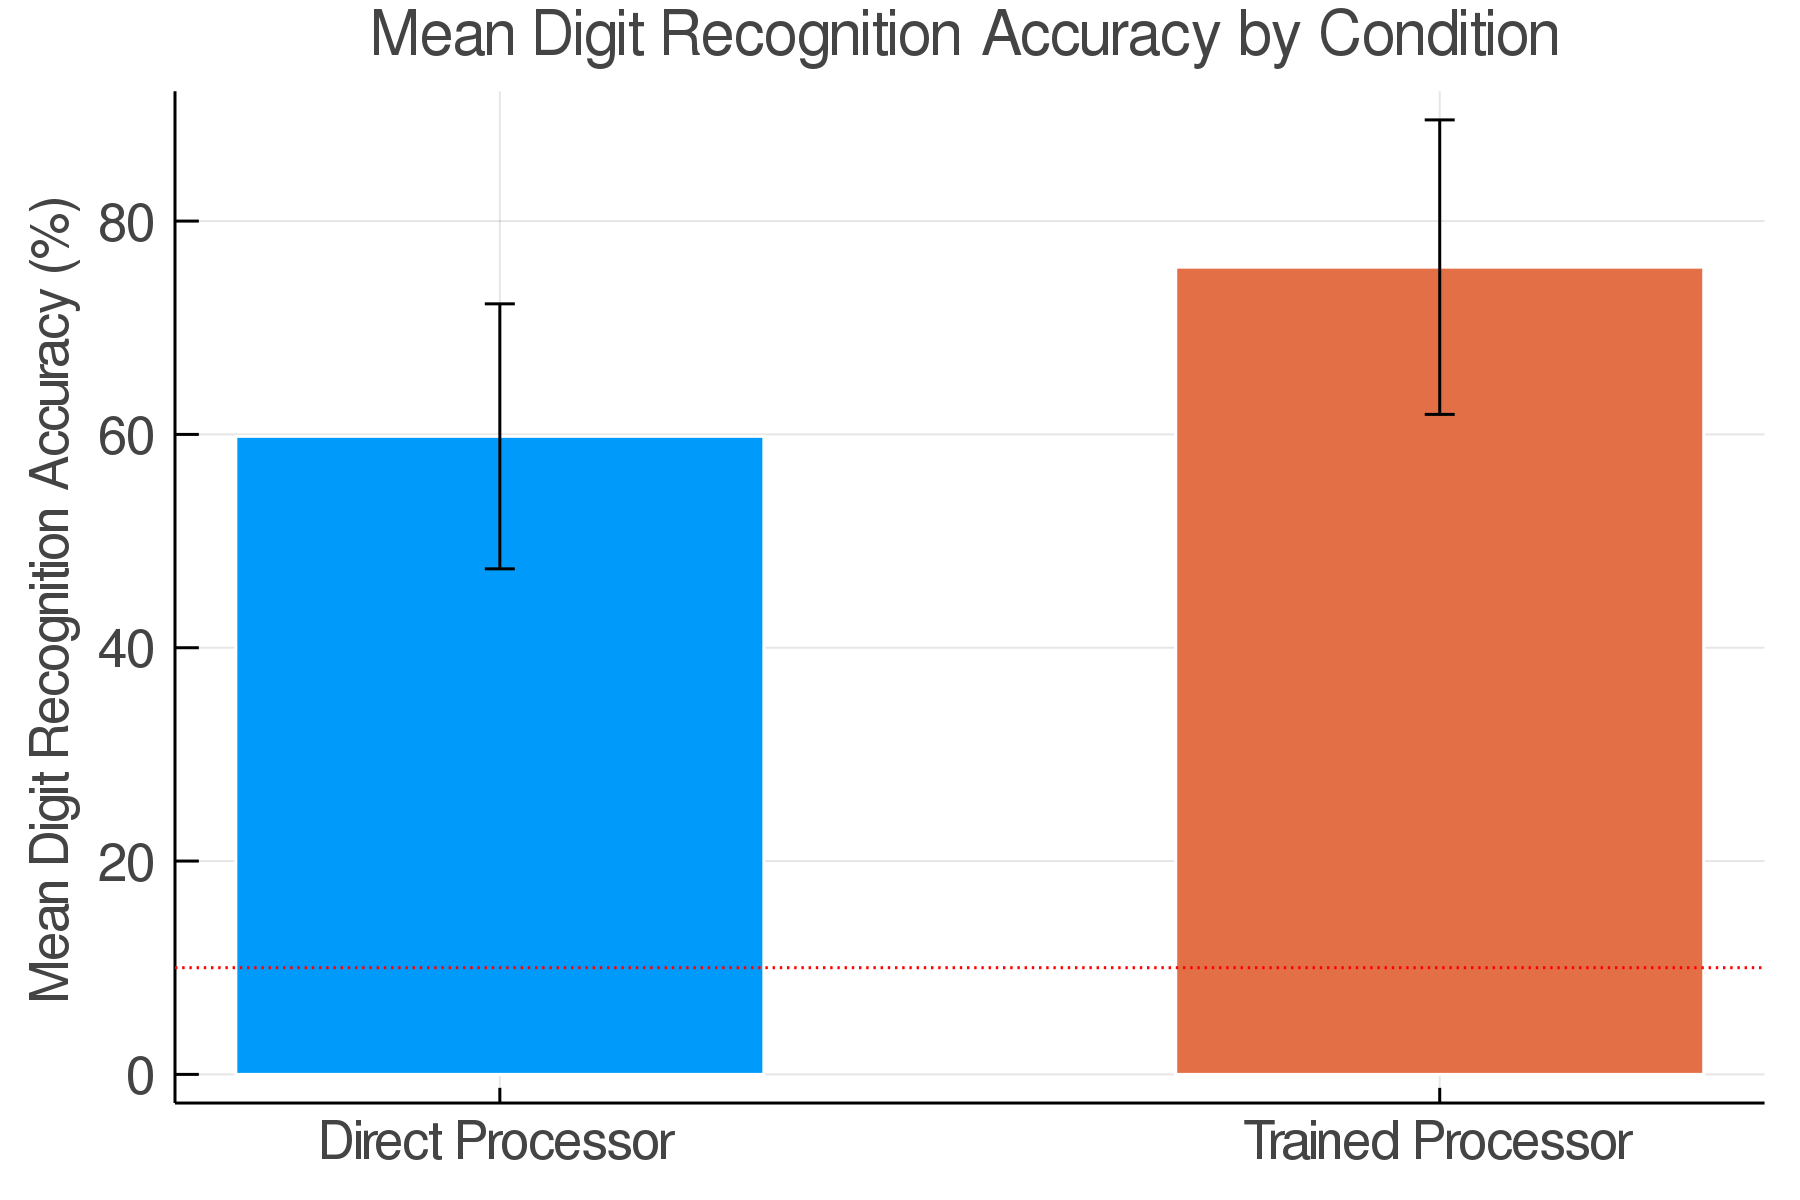
\includegraphics[width=.9\linewidth]{./images/results_mean_accuracy_overall.png}
\caption{\label{fig:org18bcdbe}
Mean digit recognition accuracy by condition, pooled participant data.}
\end{figure}


\subsection*{By Participant}
\label{sec:orgec1a690}

Of 11 participants, 9 participants performed better with the trained processor than the control processor despite variations between participants of baseline performance.
Figure \ref{fig:orgdacd8d6} compares the mean digit recognition accuracy for each condition, stratified by participant.

\begin{figure}[htbp]
\centering
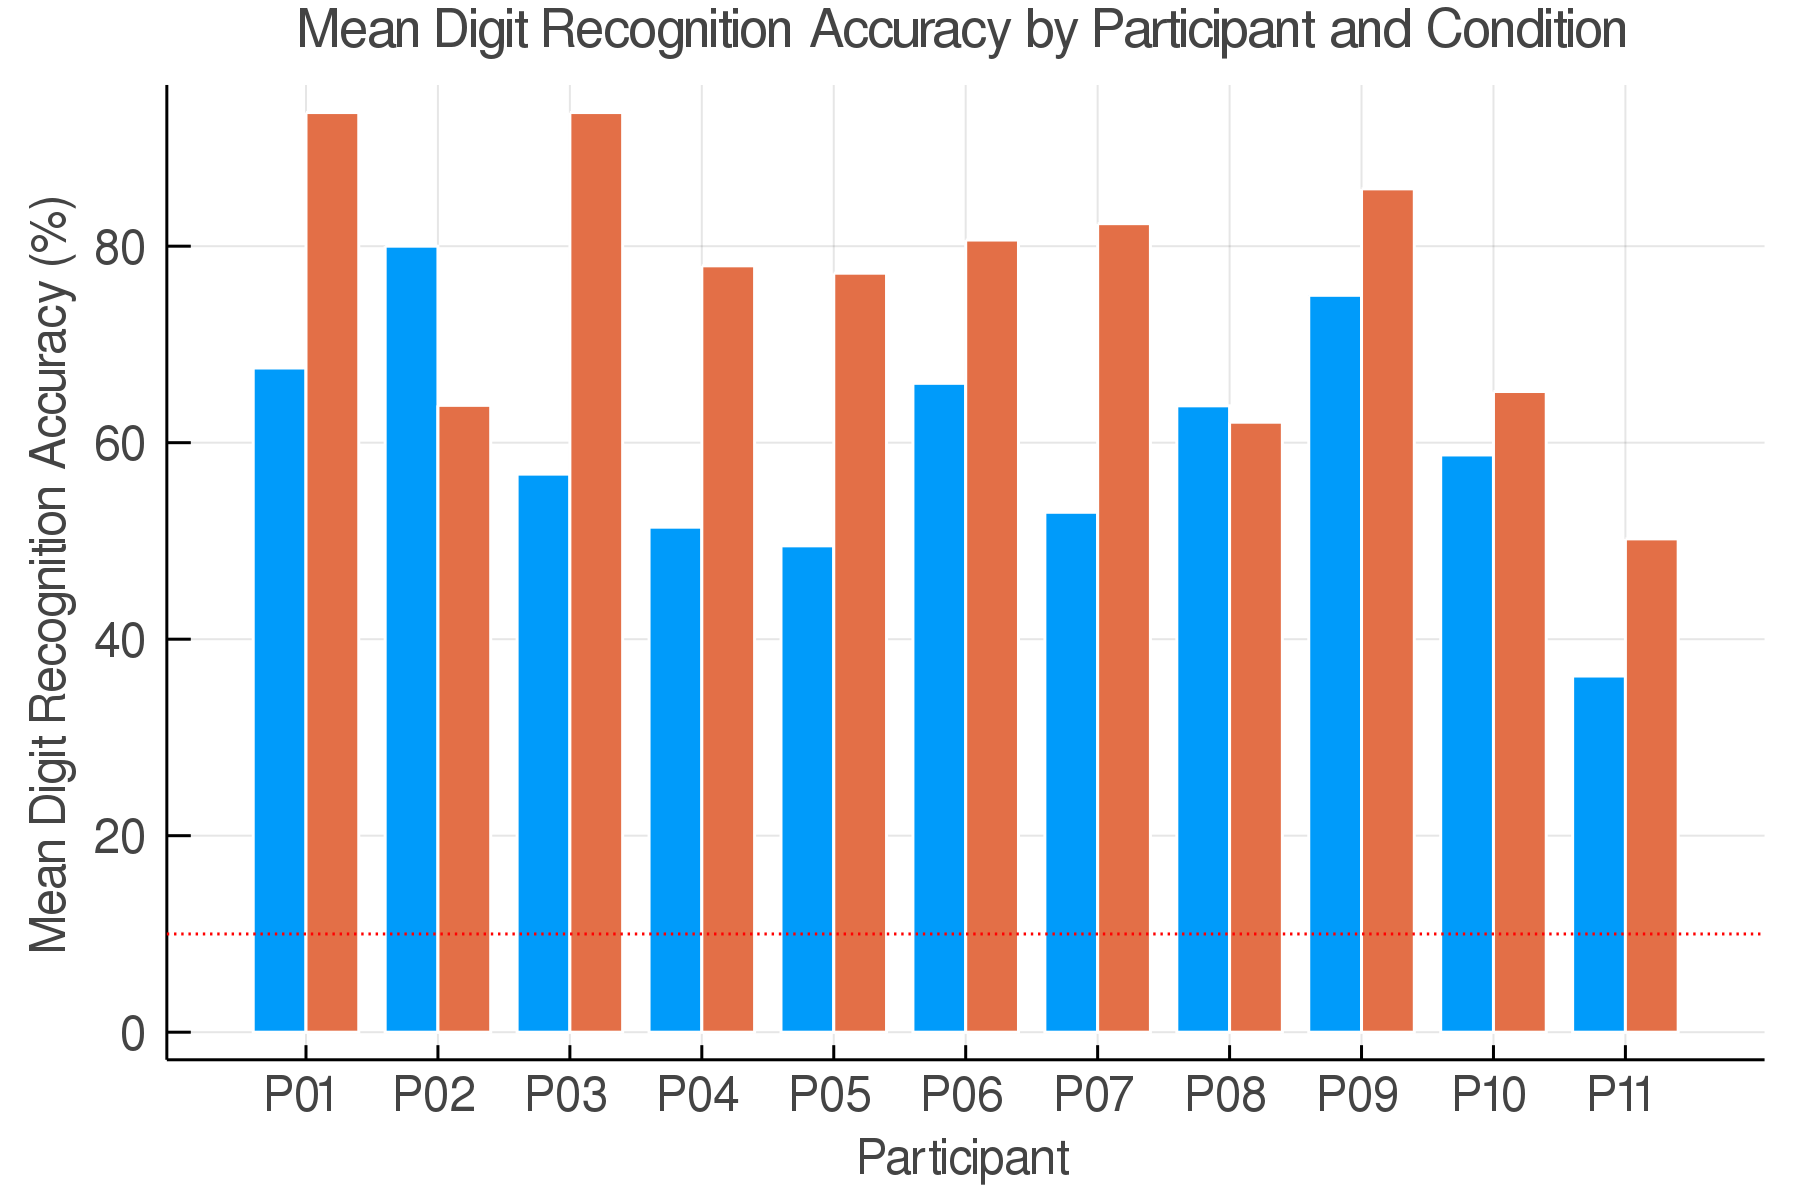
\includegraphics[width=.9\linewidth]{./images/results_mean_accuracy_by_participant.png}
\caption{\label{fig:orgdacd8d6}
Mean digit recognition accuracy by participant and condition.}
\end{figure}

\section*{Statistical Effects}
\label{sec:org44fbe40}

The correctness of participant's digit classification was modelled using logistic regression. These results are summarised in Table \ref{tab:org27c5e6e}.

\begin{table}[htbp]
\caption{\label{tab:org27c5e6e}
Predictors of a correct digit classification modelled as a logistic regression. P-values below 0.05, 0.01 and 0.001 are marked with (\texttt{*}), (\texttt{**}) and (\texttt{***}) respectively.}
\centering
\scriptsize
\begin{tabu} to \textwidth {XXXl}
\hline
Predictor & Coefficient & P-Value & Significance\\
\hline
condition & 0.959624 & <1e-77 & \texttt{***}\\
\hline
cue & 0.0184719 & 0.2237 & \\
trial & 0.176255 & <1e-12 & \texttt{***}\\
block & 0.758783 & <1e-17 & \texttt{***}\\
cue \& trial & 0.00174088 & 0.3815 & \\
cue \& block & 0.00346854 & 0.6395 & \\
trial \& block & 0.0140752 & 0.2867 & \\
cue \& trial \& block & -0.00226474 & 0.0400 & \texttt{*}\\
\hline
participant: P02 & -0.746689 & <1e-9 & \texttt{***}\\
participant: P03 & -0.391573 & 0.0016 & \texttt{**}\\
participant: P04 & -1.15042 & <1e-21 & \texttt{***}\\
participant: P05 & -1.1289 & <1e-18 & \texttt{***}\\
participant: P06 & -0.682311 & <1e-7 & \texttt{***}\\
participant: P07 & -0.914266 & <1e-12 & \texttt{***}\\
participant: P08 & -0.632393 & <1e-5 & \texttt{***}\\
participant: P09 & -0.0339482 & 0.7966 & \\
participant: P10 & -1.32654 & <1e-26 & \texttt{***}\\
participant: P11 & -2.32435 & <1e-74 & \texttt{***}\\
\hline
digit: 1 & 1.7064 & <1e-40 & \texttt{***}\\
digit: 2 & 0.233331 & 0.0300 & \texttt{*}\\
digit: 3 & 0.314268 & 0.0035 & \texttt{*}\\
digit: 4 & 0.645442 & <1e-8 & \texttt{***}\\
digit: 5 & 0.105155 & 0.3319 & \\
digit: 6 & -0.0685792 & 0.5264 & \\
digit: 7 & 1.02026 & <1e-18 & \texttt{***}\\
digit: 8 & 0.275374 & 0.0120 & \texttt{*}\\
digit: 9 & 0.065778 & 0.5451 & \\
\hline
(Intercept) & -2.08177 & <1e-20 & \texttt{***}\\
\hline
\end{tabu}
\end{table}

Figure \ref{fig:org0e1ea09} plots the same data on a scatter plot.

\begin{figure}[htbp]
\centering
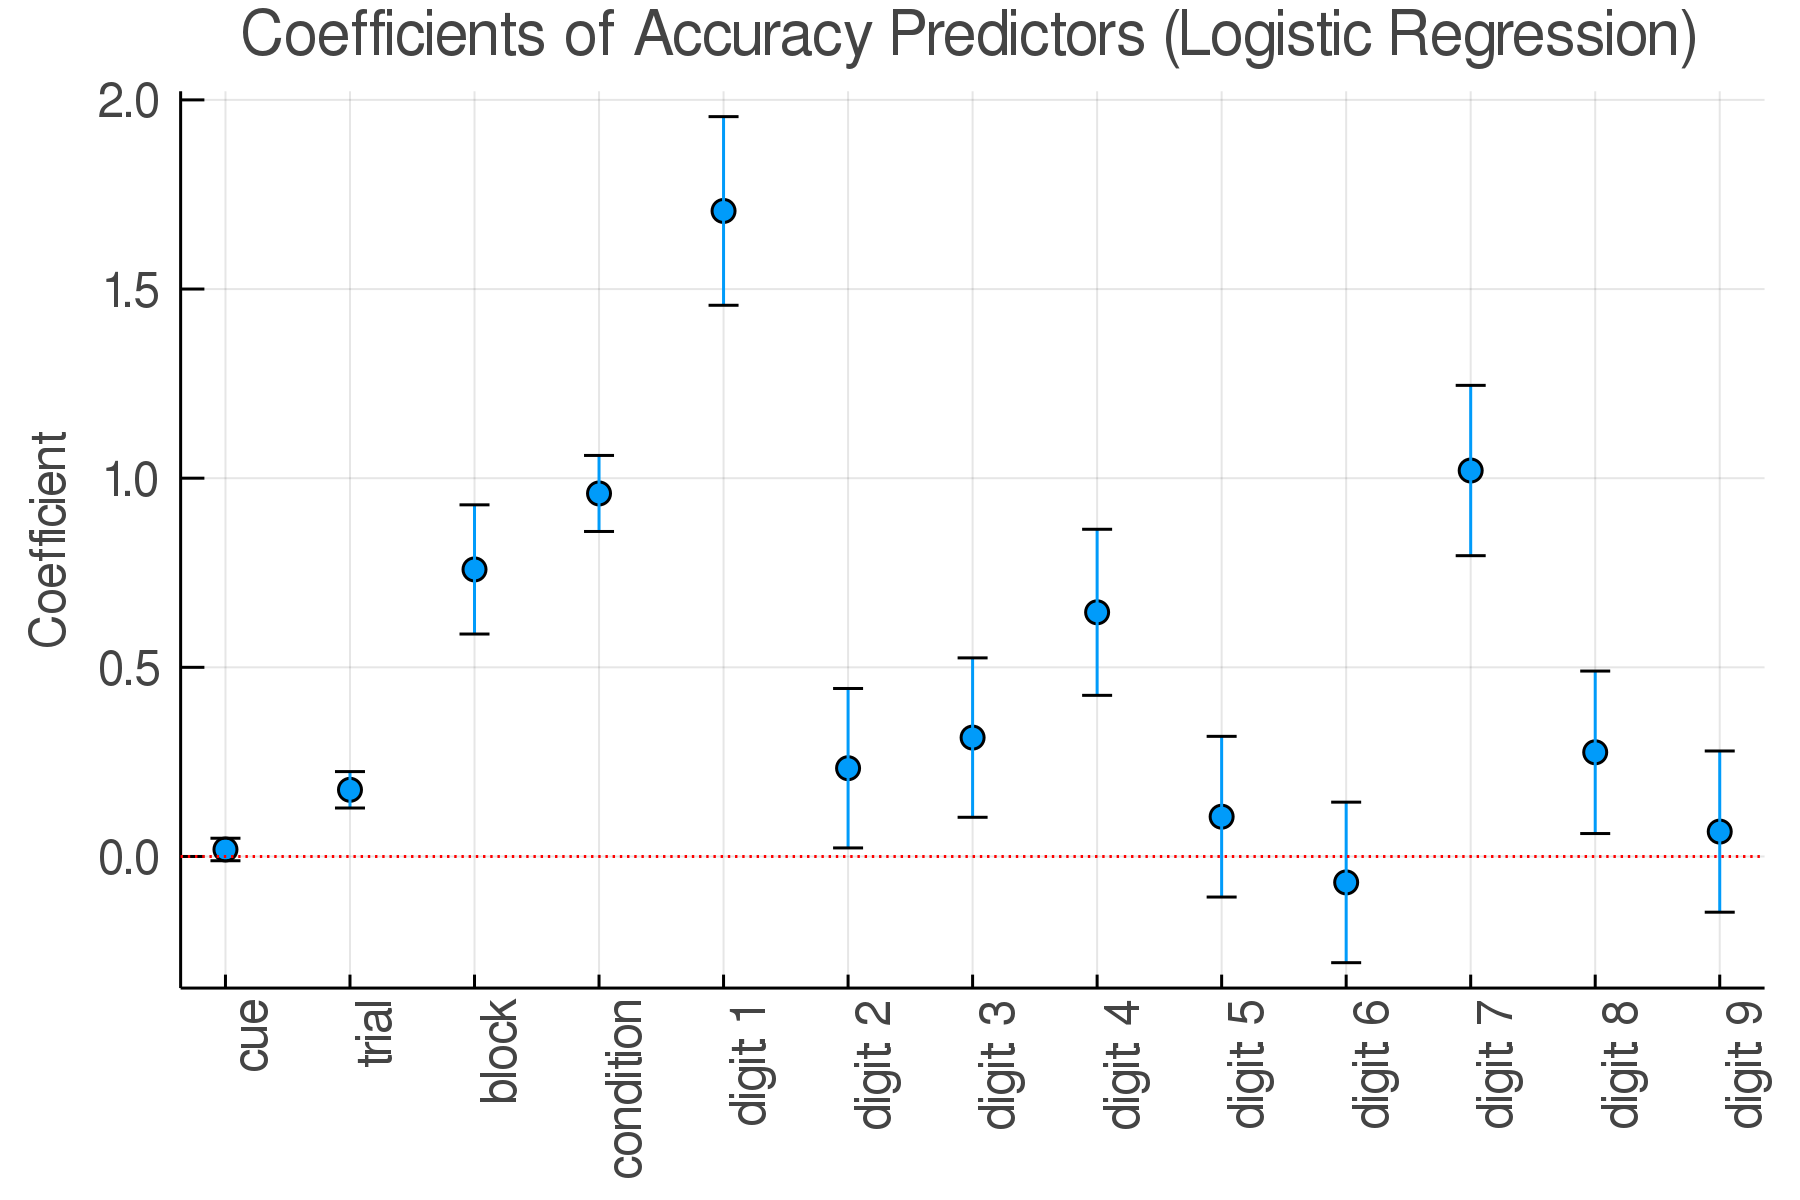
\includegraphics[width=.9\linewidth]{./images/statistical_effects.png}
\caption{\label{fig:org0e1ea09}
Predictors of a correct response in a logistic regression model. Error bars indiate 95\% confidence intervals.}
\end{figure}

\section*{Response Time}
\label{sec:org6c5d2b7}

The mean response time for a single digit was 2.6 seconds for the trained processor, versus 3.3 seconds for the trained processor.
Figure \ref{fig:org4ec77b7} shows the response time per cue for each participant.

\begin{figure}[htbp]
\centering
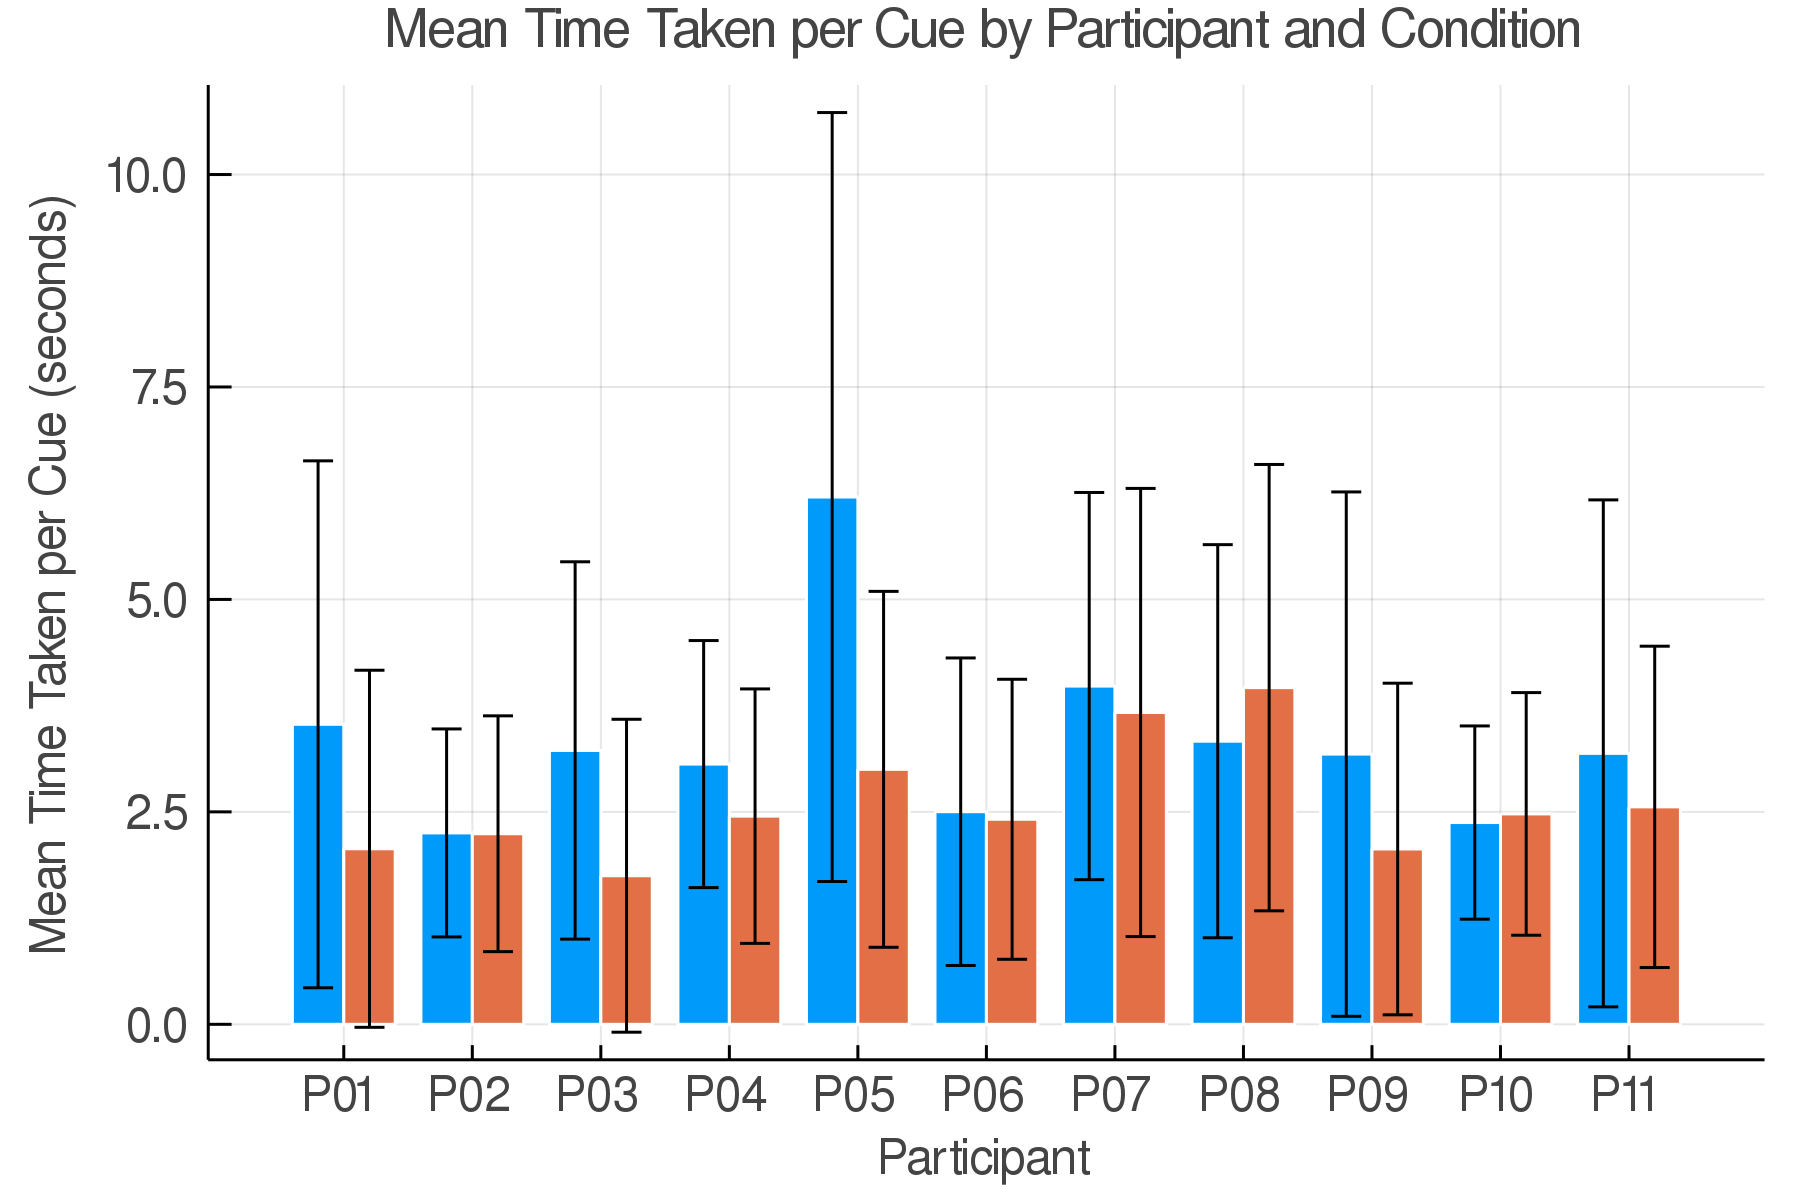
\includegraphics[width=.9\linewidth]{./images/response_time_by_participant.png}
\caption{\label{fig:org4ec77b7}
Response time per cue by participant. Error bars show standard deviation.}
\end{figure}

\section*{Learning Effects}
\label{sec:org931ea48}

Figure \ref{fig:orgdb3e0e8} shows the a rolling average with a windows size of 50 over pooled trial blocks for each condition and participant.
Participants performed with similar accuracies at the start of trial blocks, and both condition displayed a prominent learning effect.

\begin{figure}[htbp]
\centering
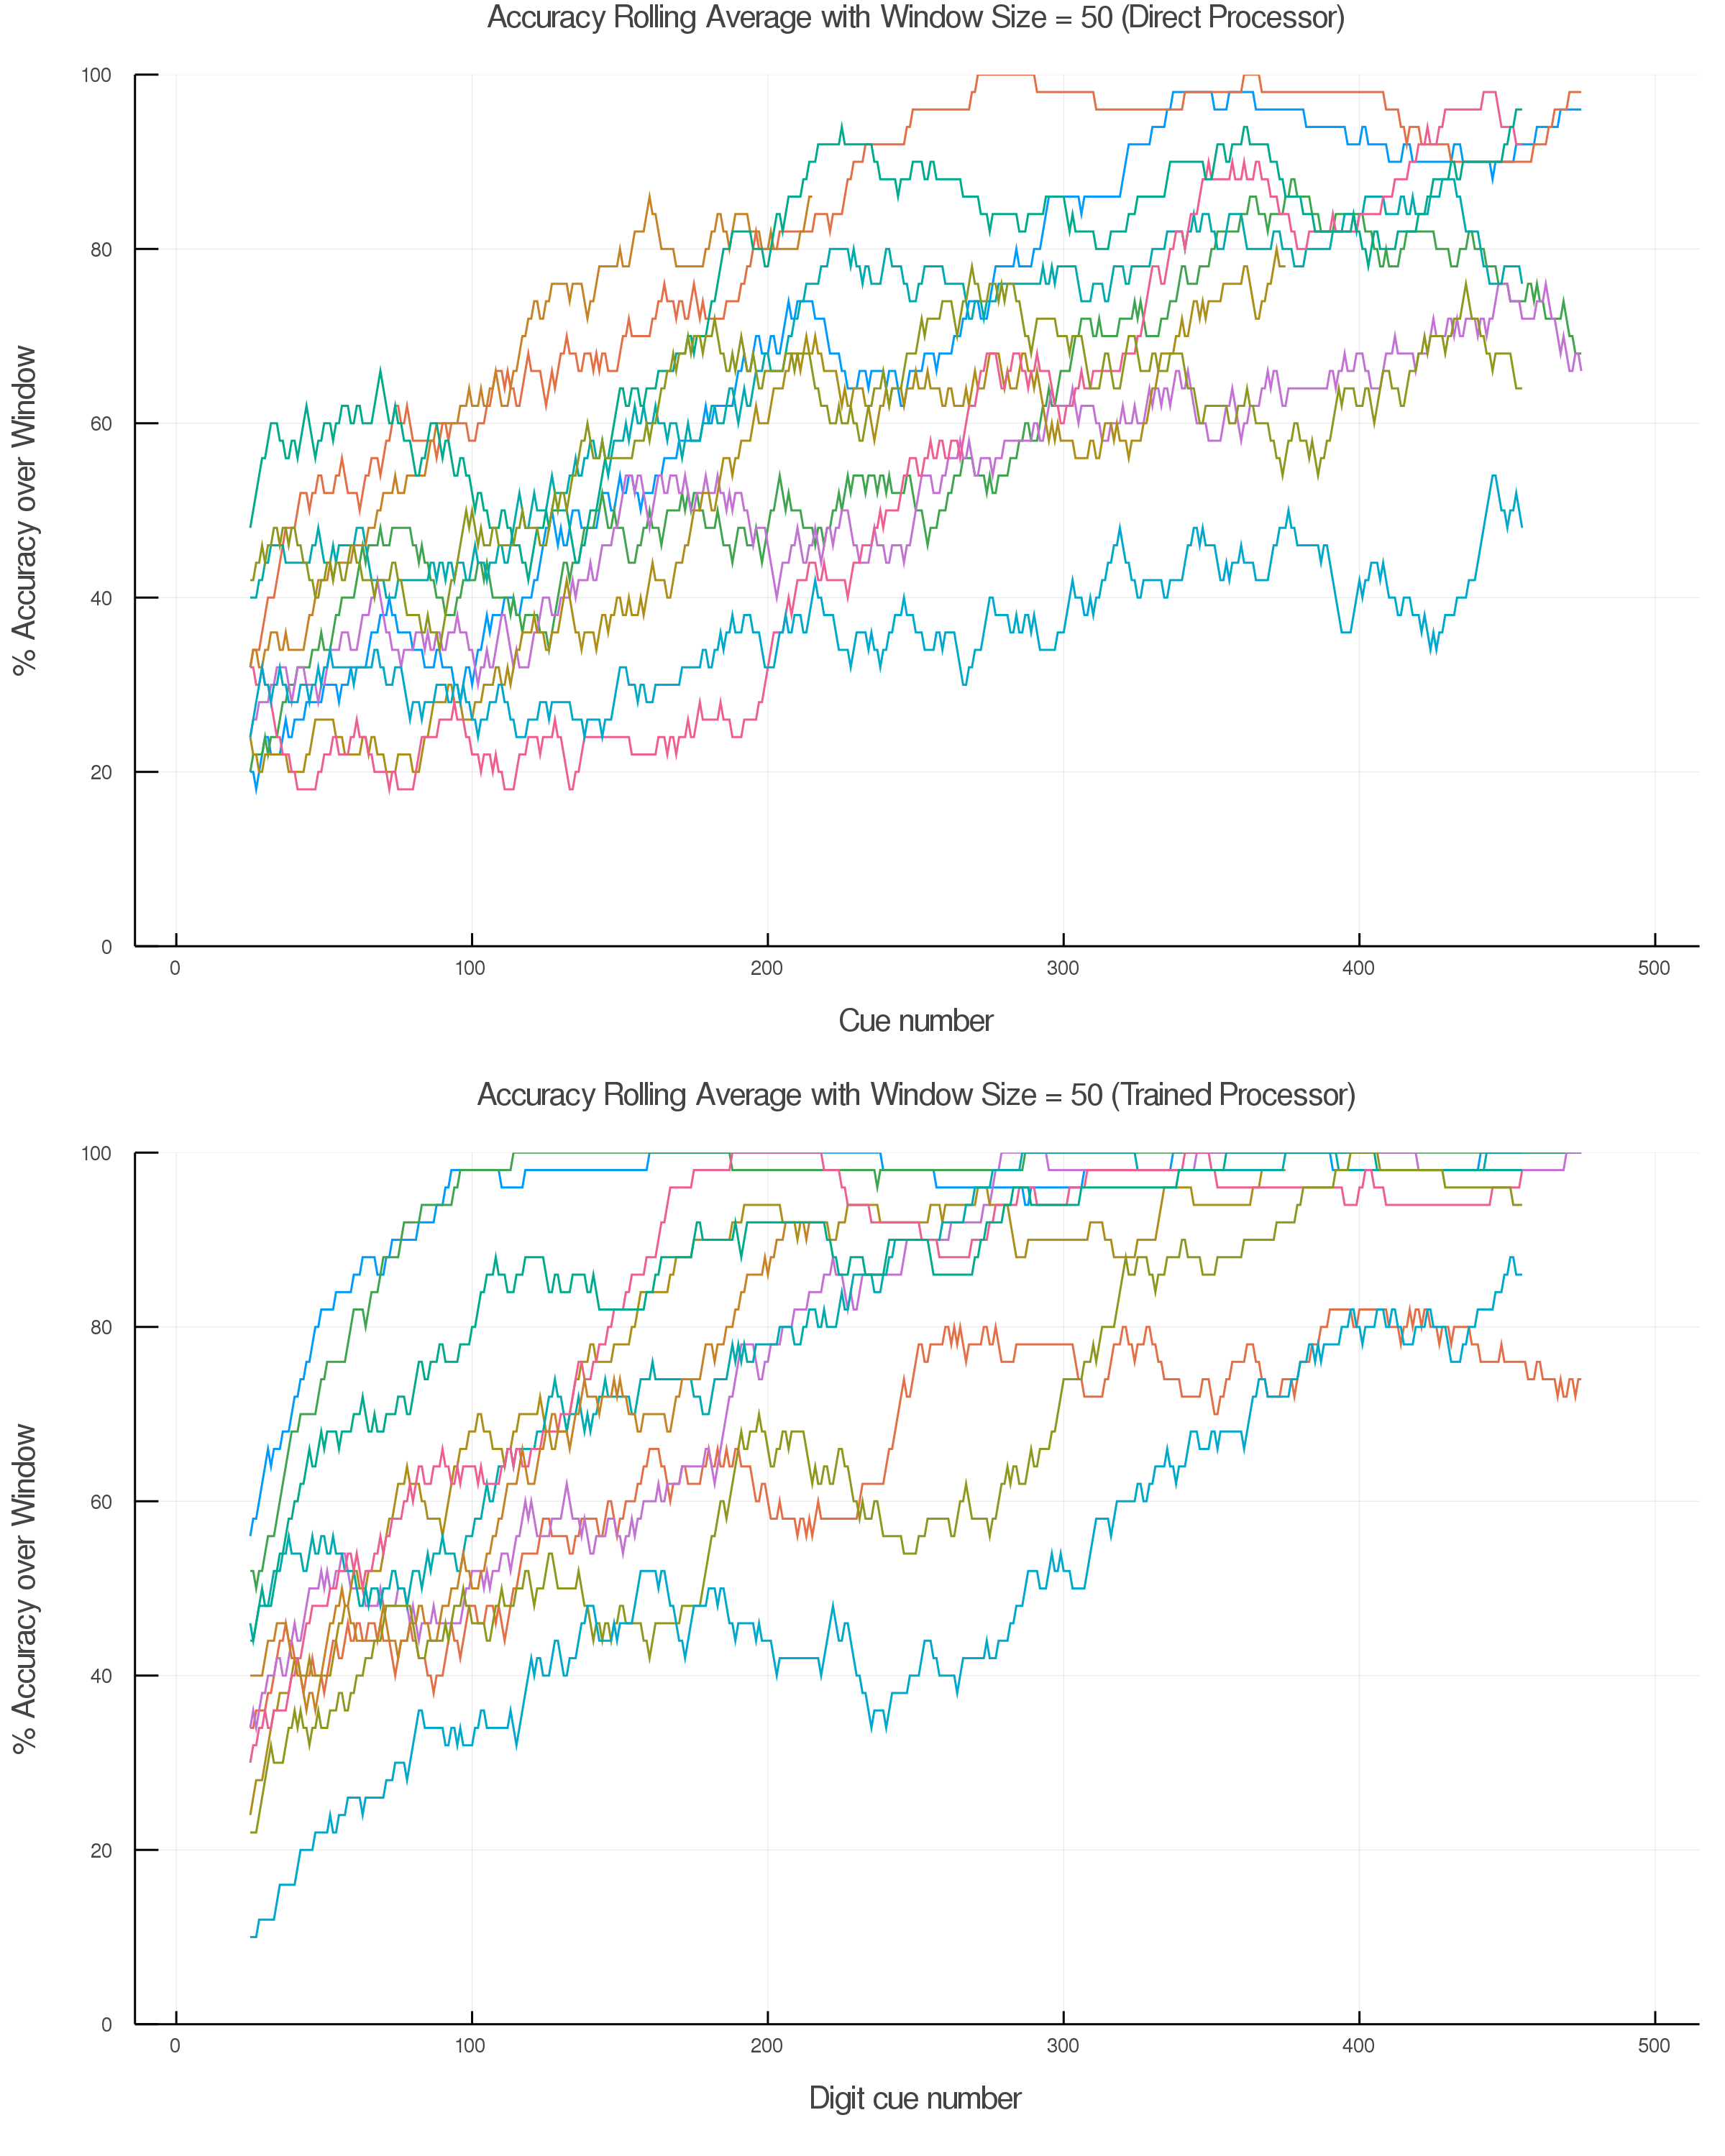
\includegraphics[width=.9\linewidth]{./images/learning_curves.png}
\caption{\label{fig:orgdb3e0e8}
Rolling average of accuracy over pooled trial blocks by condition and participant.}
\end{figure}

\begin{itemize}
\item[{$\square$}] TODO Needs more rigor, but not exactly sure how best to numerically compare it. Will think about it.
\end{itemize}

\part{Discussion}
\label{sec:orgd59c1cb}
\chapter{Aim 1: Development of GAN Training Architecture}
\label{sec:org562c76a}

A prototype GAN training architecture was successfully developed and was capable of producing phosphene encodings for different simulated grid properties.
We have approached this by implementing independent Rendering and Modification steps inside the GAN training architecture, and by allowing the Renderer be supplied different simulated phosphenes for each electrode.
In this respect, the implementation presented here serves as a proof-of-concept that a generalisable training framework is indeed possible.

Unfortunately, the output of this GAN training architecture does not always resemble their intended forms (digits).
Because this difficulty was present even in a regular Cartesian grid (which approximates pixels at higher resolutions), this is likely due to more than just intrinsic difficulties in representing digits in a grid.
Clearly, there is still a significant portion of work required before this training architecture can be considered usable for its intended purpose.

Due to the time limitations of this project, we proceeded with the psychophysics evaluation despite not achieving particularly "good-looking" digits.
Although the phosphene forms did not look like digits, it was still possible that people might find them easier to learn than the control.

\begin{itemize}
\item Write about stability!!
\begin{itemize}
\item Training data limits
\end{itemize}
\end{itemize}

\chapter{Aim 2: Psychophysics Evaluation}
\label{sec:orgabbc41e}

Participants achieved a greater overall digit classification accuracy with the trained processer versus the brightness-based control.
This effect was statistically significant when analysed using a multiple logistic regression, supporting the hypothesis that the trained processor confers better digit classification accuracy than the brightness-based control.

Notably, participant performance at the beginning of each trial block was similar between the trained and control processor.
This suggests that the trained processor phosphene forms looked no more like digits than the control processor.

It therefore appears that the better participant performance was due to a better ability to learn and distinguish the phosphene forms, rather than the the ability to find the phosphene forms immediately recognisable.



\chapter{Implications}
\label{sec:org5c73a85}

To our knowledge, this is the first attempt at tailoring phosphene patterns to specific grids through an automated process.
Although previous research has demonstrated how image processing techniques can be applied to simulated prosthetic vision, these techniques are often coupled with the simulations they run in.
This makes it hard to generalise how such techniques can be applied when the simulations strongly differ from reality.
This project, by using a dynamic simulator capable of representing arbitrary arrangements and properties of phosphenes, is therefore novel in investigating an approach to image processing decoupled from the simulation itself.

The approach we have taken in this project is an early implementation using GANs.
We have demonstrated that GANs are capable of producing digit-like forms with "high" resolution cartesian grids, though with imperfections.
This closely reflects the domain in which GANs are known to excel; where GANs have close to pixel-level access on generated images, and can optimise at a pixel-wise level.

However, we were not successful in producing reasonable digit-like forms at "low" resolution grids.
The GAN training architecture was able to produce a phosphene pattern output, but these did not resemble digits.
This is outside the domain for which GANs have previously been applied - when there is greater distance between the output of generated encodings and the simulated render.
Because GANs have not been applied in this area before, it was unknown how they would cope in this type of task.
This project therefore provides some information on the potential issues with using GANs for an encoding task with great distance between generator and renderer, as well as a basis for suggestions addressing these issues.

A prominent issue arising from this project is how to evaluate how intrinsically capable different grids are for representing recognisable digits.
It is not altogether clear whether the issues with representing digits arose due to limitations of the GAN architecture, or the impossibility of representing digits for some types of grids in the first place.
A contrived example is where a grid is composed of phosphenes arranged entirely in a single vertical line; it would be impossible to make any recognisable digit from this grid except for a digit 1.
This is especially a problem with low-resolution grids with other distortions (such as size variance), where the contribution and valuability of each phosphene is relatively high.
This problem - the lack of a means of evaluating the informative capacity of different phosphene grids - has not previously been addressed.

Nevertheless, we have demonstrated that computer-generated phosphene forms may still be useful to improve the discriminability of phosphene patterns, even though they do not look like digits.
The results of our psychophysics experiment, which we undertook at low-resolution, irregular and distorted grids, demonstrate that although people did not recognise the forms as digits, they were able to learn their meanings better than a direct mask-based control.
There is no doubt that manually-crafted phosphene patterns would have easily surpassed the performance of our GAN implementation as it currently stands.
However, the usefulness of this GAN implementation is that it is an automated process, and not exclusive to digit forms (provided there is training data of other forms which you wish to represent).
There is therefore an advantage to refining automated processes of generating phosphene forms rather than relying on the ability of humans to manually craft phosphene patterns representing digits.

The current results of this project are not compelling for, nor against, the use of GANs in addressing the perceptual limitations of prosthetic vision.
We have demonstrated how a GAN can be implemented to perform a phosphene generation task for different simulated grids, and how this performance varies with different simulated properties.
The GAN was not robust against all different simulated properties.

\chapter{Limitations}
\label{sec:org54495c3}

\section*{Simulated Prosthetic Vision}
\label{sec:orgeabbf8c}

One of the criticisms highlighted in the Background section was the difficulty of dealing with differences between simulated prosthetic vision and prosthetic vision \emph{in vivo}.
While this project addresses one of these differences - coping with different \emph{spatial} phosphene properties - many differences remain for which the translation of techniques from simulated space to \emph{in vivo} space is unclear.
These include:
\begin{enumerate}
\item \textbf{Temporal qualities of phosphenes, such as flickering and dimming over time}.
This is important in understanding how vision can be provided to implantees continuously like natural vision, and how temporal properties could be used to improve implantees' visual understanding.
Our training implementation does not currently allow for producing or testing anything more than static patterns.
Notably however, static patterns are not necessarily a poor choice since continuously-changing phosphene patterns might provoke confusion in implantees, particularly in low-resolution implants as is currently expected.
\item \textbf{Effects of simultaneously eliciting phosphenes.}
In this experiment, simultaneously stimulated phosphenes were shown simultaneously for simplicity; however, empirical evidence suggests that simultaneously elicited phosphenes may not combine additively.
This aspect of the simulation could theoretically be incorporated in our GAN training architecture, but was not trialled in this experiment.
\item \textbf{The movement of phosphenes with eye movements.}
Phosphenes are known to move with eye movements, meaning that peripheral phosphenes would always be perceived peripherally.
Our psychophysics experiment did not incorporate eye movement tracking as it was intended purely as a preliminary validation measure rather than a true test of applicability.
Participants were therefore able to scan and study phosphene patterns, which may not be possible \emph{in vivo}.
This feature could, however, be modelled in a future experiment with greater resources and refinement of phosphene patterns as a stronger test of applicability.
\end{enumerate}

The results presented here should therefore still be considered within the context of simulated prosthetic vision and all its caveats, as it primarily focused on addressing one particular issue of simulated prosthetic vision rather than all.

\section*{Experimental Features}
\label{sec:org69d5c00}

The sample size of the psychophysics experiment used in this project was notably small with 11 participants only.
The rationale for this sample size was that it served as an intermediate checkpoint to point-out weaknesses in the current architecture and guide further development.
The investment required for recruiting and conducting the experiment on more participants was not justified by the status of the GAN implementation as an early prototype.
However, should the prototype be further developed, it is important to validate in a greater number of participants.

\begin{itemize}
\item Somehow talk sbout simulated
\end{itemize}

\section*{Choice of Task}
\label{sec:org5f8d097}

The digit recognition task in this experiment was chosen to optimise data collection so as many data samples could be collected as possible from each participant.
The task - recognising a single digit known to belong to the class of 0-9 - is therefore extremely simple and somewhat contrived.

The use of a simple, constrained task was necessary for this project as it investigated a single feature - the discriminability of phosphene patterns.
At the current stage of implementation, it is not as informative for development to use "natural" tasks - such as navigation, reading or unconstrained object identification - which often incorporate multiple aspects of visual information as well as other senses.
However, the reality is that natural visual tasks are of greatest interest to future implantees.
Whilst in early development, the use of simple, constrained tasks is crucial to directly highlight strengths and weaknesses of image processing techniques, these must eventually be tested in more natural environments.
This project is not yet at that stage.

\begin{itemize}
\item ALSO comment on qualitative limitations - e.g. requirement for training/resources,
\item Maybe also comment on choice of comparison?
\end{itemize}

\chapter{Future Directions}
\label{sec:org534d2c4}

Given that this is a prototypical implementation, it is important that the results of this work can be used to improve research on the use of GANs in simulated prosthetic vision even though the early results are not conclusive.

\section*{Training Data}
\label{sec:org02b7c7c}

We used MNIST digits as the source of real digits for our training implementation and modified them slightly to suit the visual properties of our simulation.
We also attempted to bring the renders closer to the domain of MNIST digits using a style-transfer network to "fill holes" in the phosphene and extract forms.

However it does not appear our measures were enough for the network to remain stable.
It was evident from the training loss curves that the \emph{Generator} was never able to fool the \emph{Discriminator} reliably.
As a result, the \emph{Generator}'s produced encodings often drifted rather than converging to an optimal solution.

An easy improvement to make (and one which does not require changing the actual training architecture itself) is to use digit forms closer to the image domain of simulated renders as training data.
This could be sourced by creating

In addition, training data representing other forms could be used instead, such as outlines of common objects (such as chairs) or letterforms.
Using different forms of training data does not require any major changes to the architecture, as the training data is not part of the architecture itself (and therefore can simply be "mixed and matched").
A potential source of outline data is the Google Quick, Draw! Dataset, which contains millions of simple, line-based drawings of objects and animals.
As the ability to substitute different forms of training data is one of the benefits of using GANs, this could potentially provide further information on whether GANs are justified for simulated prosthetic vision.

\section*{Grid Evaluation}
\label{sec:org8750e9c}

This project faced major difficulties in creating recognisable phosphene patterns for low-resolution distorted grids.
Part of this difficulty is due to intrinsic limitations on \emph{what} can be represented on grids with a small quantity of phosphenes.
Certain types of grid, such as a single linear "grid" of phosphenes, clearly constrain the types of shapes that can be represented.

It would be informative and time-saving to be able to evaluate grids beforehand to quantify their usefulness for representing specific types of phosphene patterns.
This could be as simple as a measure of dispersion of phosphenes in 2D space for simple grid simulations.
There is scant literature on the use of image processing techniques for grid resolutions as low as those tested in this project (64 phosphenes), which may partially be why this has not previously been an issue.
However, given that first-generation CVPs are only designed to produce up to a maximum of 473 phosphenes (with most implants far below this number), being able to quantify phosphene grids' representability would be useful for early \emph{in vivo} experiments.

\part{Conclusion}
\label{sec:org75550c3}

This project has explored how generative adversarial networks (GANs) may be used to generate phosphene patterns for arbitrary simulated properties of prosthetic vision, and to our knowledge is the first attempt at addressing phosphene pattern generation decoupled from simulation properties. 
We developed a prototypical software implementation of a GAN training architecture to generate phosphene patterns of digits, and tested whether these helped people recognise digits in a psychophysics experiment compared to a mask-based control.
The early training implementation we developed was successfully able to produce phosphene digit patterns for different grid properties including phosphene distribution, sizing and resolution.
However, the produced phosphene digit patterns were only recognisable as digits at high grid resolutions and not at low grid resolutions, and the generated patterns proved unstable over epochs.
Nevertheless, at low resolution, participants were still able to learn the generated phosphene patterns better than the mask-based control and achieved a higher recognition accuracy overall.
The results of this checkpoint suggest that the current GAN implementation may be helpful in increasing the discriminability of phosphene patterns for a simple classification task, but are not yet robust against low-resolution grids and spatial distortions.
This project provides useful information on potential targets for improving a GAN implementation; further work should focus on improving the stability of GAN training and quantifying intrinsic capabilities of low-resolution grids to represent form-based information.

\begin{appendices}
\part{Appendices}
\label{sec:org1ba2208}
\chapter{Additional Qualitative Results: Examples}
\label{sec:org2107f69}
\chapter{Psychophysics Explanatory Statement}
\label{sec:orgfb36cef}
\chapter{Selected Code}
\label{sec:org7fd5dd3}
\section*{Psychophysics Experiment}
\label{sec:orgbba68cf}
\section*{Plotting}
\label{sec:orged761fc}
\clearpage
\part{References}
\label{sec:orgf74fed5}
\bibliographystyle{vancouver}
\bibliography{refs}
\end{appendices}
\end{document}
